% ****** Start of file apssamp.tex ******
%
%   This file is part of the APS files in the REVTeX 4.2 distribution.
%   Version 4.2a of REVTeX, December 2014
%
%   Copyright (c) 2014 The American Physical Society.
%
%   See the REVTeX 4 README file for restrictions and more information.
%
% TeX'ing this file requires that you have AMS-LaTeX 2.0 installed
% as well as the rest of the prerequisites for REVTeX 4.2
%
% See the REVTeX 4 README file
% It also requires running BibTeX. The commands are as follows:
%
%  1)  latex apssamp.tex
%  2)  bibtex apssamp
%  3)  latex apssamp.tex
%  4)  latex apssamp.tex
%
\documentclass[%
 reprint,
superscriptaddress,
%groupedaddress,
%unsortedaddress,
%runinaddress,
%frontmatterverbose, 
%preprint,
%preprintnumbers,
%nofootinbib,
%nobibnotes,
%bibnotes,
 amsmath,amssymb,
 aps,
%pra,
%prb,
%rmp,
%prstab,
%prstper,
%floatfix,
]{revtex4-2}

\usepackage{graphicx}% Include figure files
\usepackage{dcolumn}% Align table columns on decimal point
\usepackage{bm}% bold math
%\usepackage{hyperref}% add hypertext capabilities
%\usepackage[mathlines]{lineno}% Enable numbering of text and display math
%\linenumbers\relax % Commence numbering lines

%\usepackage[showframe,%Uncomment any one of the following lines to test 
%%scale=0.7, marginratio={1:1, 2:3}, ignoreall,% default settings
%%text={7in,10in},centering,
%%margin=1.5in,
%%total={6.5in,8.75in}, top=1.2in, left=0.9in, includefoot,
%%height=10in,a5paper,hmargin={3cm,0.8in},
%]{geometry}


\begin{document}

\preprint{APS/NBrS}

\title{First evidence of Neutral Bremsstrahlung emission in xenon} % Force line breaks with \\
%\thanks{A footnote to the article title}%

\author{C.A.O.~Henriques}
\email[Corresponding authors, ]{cristinam@uc.pt, henriques@uc.pt}
\affiliation{LIBPhys, Physics Department, University of Coimbra, Rua Larga, Coimbra, 3004-516, Portugal}%

\author{P.~Amedo}
\affiliation{Instituto Gallego de F\'isica de Altas Energ\'ias, Univ.\ de Santiago de Compostela, Campus sur, R\'ua Xos\'e Mar\'ia Su\'arez N\'u\~nez, s/n, Santiago de Compostela, E-15782, Spain}%

\author{J.M.R.~Teixeira}
\affiliation{LIBPhys, Physics Department, University of Coimbra, Rua Larga, Coimbra, 3004-516, Portugal}%

\author{D.~Gonz\'alez-D\'iaz}
\affiliation{Instituto Gallego de F\'isica de Altas Energ\'ias, Univ.\ de Santiago de Compostela, Campus sur, R\'ua Xos\'e Mar\'ia Su\'arez N\'u\~nez, s/n, Santiago de Compostela, E-15782, Spain}%

\author{C.D.R.~Azevedo}
\affiliation{Institute of Nanostructures, Nanomodelling and Nanofabrication (i3N), Universidade de Aveiro, Campus de Santiago, Aveiro, 3810-193, Portugal}%

\author{A.~Para} 
\affiliation{Fermi National Accelerator Laboratory, Batavia, IL 60510, USA}%

\author{J.~Mart\'in-Albo}
\affiliation{Instituto de F\'isica Corpuscular (IFIC), CSIC \& Universitat de Val\`encia, Calle Catedr\'atico Jos\'e Beltr\'an, 2, Paterna, E-46980, Spain}%

\author{A. Saa Hernandez}
\affiliation{Instituto Gallego de F\'isica de Altas Energ\'ias, Univ.\ de Santiago de Compostela, Campus sur, R\'ua Xos\'e Mar\'ia Su\'arez N\'u\~nez, s/n, Santiago de Compostela, E-15782, Spain}%

\author{J.J.~G\'omez-Cadenas}
\thanks{NEXT Co-spokesperson.}
\affiliation{Donostia International Physics Center (DIPC), Paseo Manuel Lardizabal, 4, Donostia-San Sebastian, E-20018, Spain}%
\affiliation{Ikerbasque, Basque Foundation for Science, Bilbao, E-48013, Spain}%

\author{D.R.~Nygren}
\thanks{NEXT Co-spokesperson.}
\affiliation{Department of Physics, University of Texas at Arlington, Arlington, TX 76019, USA}%

\author{C.M.B.~Monteiro}
\email[Corresponding authors, ]{cristinam@uc.pt, henriques@uc.pt}
\affiliation{LIBPhys, Physics Department, University of Coimbra, Rua Larga, Coimbra, 3004-516, Portugal}%

\author{C.~Adams}
\affiliation{Argonne National Laboratory, Argonne, IL 60439, USA}%

\author{V.~\'Alvarez}
\affiliation{Instituto de Instrumentaci\'on para Imagen Molecular (I3M), Centro Mixto CSIC - Universitat Polit\`ecnica de Val\`encia, Camino de Vera s/n, Valencia, E-46022, Spain}%

\author{L.~Arazi}
\affiliation{Nuclear Engineering Unit, Faculty of Engineering Sciences, Ben-Gurion University of the Negev, P.O.B. 653, Beer-Sheva, 8410501, Israel}%

\author{I.J.~Arnquist}
\affiliation{Pacific Northwest National Laboratory (PNNL), Richland, WA 99352, USA}%

\author{K.~Bailey}
\affiliation{Argonne National Laboratory, Argonne, IL 60439, USA}%

\author{F.~Ballester}
\affiliation{Instituto de Instrumentaci\'on para Imagen Molecular (I3M), Centro Mixto CSIC - Universitat Polit\`ecnica de Val\`encia, Camino de Vera s/n, Valencia, E-46022, Spain}%

\author{J.M.~Benlloch-Rodr\'{i}guez}
\affiliation{Donostia International Physics Center (DIPC), Paseo Manuel Lardizabal, 4, Donostia-San Sebastian, E-20018, Spain}%
\affiliation{Instituto de F\'isica Corpuscular (IFIC), CSIC \& Universitat de Val\`encia, Calle Catedr\'atico Jos\'e Beltr\'an, 2, Paterna, E-46980, Spain}%

\author{F.I.G.M.~Borges}
\affiliation{LIP, Department of Physics, University of Coimbra, Coimbra, 3004-516, Portugal}%

\author{N.~Byrnes}
\affiliation{Department of Physics, University of Texas at Arlington, Arlington, TX 76019, USA}%

\author{S.~C\'arcel}
\affiliation{Instituto de F\'isica Corpuscular (IFIC), CSIC \& Universitat de Val\`encia, Calle Catedr\'atico Jos\'e Beltr\'an, 2, Paterna, E-46980, Spain}%

\author{J.V.~Carri\'on}
\affiliation{Instituto de F\'isica Corpuscular (IFIC), CSIC \& Universitat de Val\`encia, Calle Catedr\'atico Jos\'e Beltr\'an, 2, Paterna, E-46980, Spain}%

\author{S.~Cebri\'an}
\affiliation{Centro de Astropart\'iculas y F\'isica de Altas Energ\'ias (CAPA), Universidad de Zaragoza, Calle Pedro Cerbuna, 12, Zaragoza, E-50009, Spain}%

\author{E.~Church}
\affiliation{Pacific Northwest National Laboratory (PNNL), Richland, WA 99352, USA}%

\author{C.A.N.~Conde}
\affiliation{LIP, Department of Physics, University of Coimbra, Coimbra, 3004-516, Portugal}%

\author{T.~Contreras}
\affiliation{Department of Physics, Harvard University, Cambridge, MA 02138, USA}%

\author{G.~D\'iaz}
\affiliation{Instituto Gallego de F\'isica de Altas Energ\'ias, Univ.\ de Santiago de Compostela, Campus sur, R\'ua Xos\'e Mar\'ia Su\'arez N\'u\~nez, s/n, Santiago de Compostela, E-15782, Spain}%

\author{J.~D\'iaz}
\affiliation{Instituto de F\'isica Corpuscular (IFIC), CSIC \& Universitat de Val\`encia, Calle Catedr\'atico Jos\'e Beltr\'an, 2, Paterna, E-46980, Spain}%

\author{M.~Diesburg}
\affiliation{Fermi National Accelerator Laboratory, Batavia, IL 60510, USA}%

\author{J.~Escada}
\affiliation{LIP, Department of Physics, University of Coimbra, Coimbra, 3004-516, Portugal}%

\author{R.~Esteve}
\affiliation{Instituto de Instrumentaci\'on para Imagen Molecular (I3M), Centro Mixto CSIC - Universitat Polit\`ecnica de Val\`encia, Camino de Vera s/n, Valencia, E-46022, Spain}%

\author{R.~Felkai}
\affiliation{Nuclear Engineering Unit, Faculty of Engineering Sciences, Ben-Gurion University of the Negev, P.O.B. 653, Beer-Sheva, 8410501, Israel}%
\affiliation{Nuclear Research Center Negev, Beer-Sheva, 84190, Israel}%
\affiliation{Instituto de F\'isica Corpuscular (IFIC), CSIC \& Universitat de Val\`encia, Calle Catedr\'atico Jos\'e Beltr\'an, 2, Paterna, E-46980, Spain}%

\author{A.F.M.~Fernandes}
\affiliation{LIBPhys, Physics Department, University of Coimbra, Rua Larga, Coimbra, 3004-516, Portugal}%

\author{L.M.P.~Fernandes}
\affiliation{LIBPhys, Physics Department, University of Coimbra, Rua Larga, Coimbra, 3004-516, Portugal}%

\author{P.~Ferrario}
\affiliation{Donostia International Physics Center (DIPC), Paseo Manuel Lardizabal, 4, Donostia-San Sebastian, E-20018, Spain}%
\affiliation{Ikerbasque, Basque Foundation for Science, Bilbao, E-48013, Spain}%

\author{A.L.~Ferreira}
\affiliation{Institute of Nanostructures, Nanomodelling and Nanofabrication (i3N), Universidade de Aveiro, Campus de Santiago, Aveiro, 3810-193, Portugal}%

\author{E.D.C.~Freitas}
\affiliation{LIBPhys, Physics Department, University of Coimbra, Rua Larga, Coimbra, 3004-516, Portugal}%

\author{J.~Generowicz}
\affiliation{Donostia International Physics Center (DIPC), Paseo Manuel Lardizabal, 4, Donostia-San Sebastian, E-20018, Spain}%

\author{S.~Ghosh}
\affiliation{Department of Physics, Harvard University, Cambridge, MA 02138, USA}%

\author{A.~Goldschmidt}
\affiliation{Lawrence Berkeley National Laboratory (LBNL), 1 Cyclotron Road, Berkeley, CA 94720, USA}%

\author{R.~Guenette}
\affiliation{Department of Physics, Harvard University, Cambridge, MA 02138, USA}%

\author{R.M.~Guti\'errez}
\affiliation{Centro de Investigaci\'on en Ciencias B\'asicas y Aplicadas, Universidad Antonio Nari\~no, Sede Circunvalar, Carretera 3 Este No.\ 47 A-15, Bogot\'a, Colombia}%

\author{J.~Haefner}
\affiliation{Department of Physics, Harvard University, Cambridge, MA 02138, USA}%

\author{K.~Hafidi}
\affiliation{Argonne National Laboratory, Argonne, IL 60439, USA}%

\author{J.~Hauptman}
\affiliation{Department of Physics and Astronomy, Iowa State University, 12 Physics Hall, Ames, IA 50011-3160, USA}%

\author{J.A.~Hernando~Morata}
\affiliation{Instituto Gallego de F\'isica de Altas Energ\'ias, Univ.\ de Santiago de Compostela, Campus sur, R\'ua Xos\'e Mar\'ia Su\'arez N\'u\~nez, s/n, Santiago de Compostela, E-15782, Spain}%

\author{P.~Herrero}
\affiliation{Donostia International Physics Center (DIPC), Paseo Manuel Lardizabal, 4, Donostia-San Sebastian, E-20018, Spain}%

\author{V.~Herrero}
\affiliation{Instituto de Instrumentaci\'on para Imagen Molecular (I3M), Centro Mixto CSIC - Universitat Polit\`ecnica de Val\`encia, Camino de Vera s/n, Valencia, E-46022, Spain}%

\author{Y.~Ifergan}
\affiliation{Nuclear Engineering Unit, Faculty of Engineering Sciences, Ben-Gurion University of the Negev, P.O.B. 653, Beer-Sheva, 8410501, Israel}%
\affiliation{Nuclear Research Center Negev, Beer-Sheva, 84190, Israel}%

\author{S.~Johnston}
\affiliation{Argonne National Laboratory, Argonne, IL 60439, USA}%

\author{B.J.P.~Jones}
\affiliation{Department of Physics, University of Texas at Arlington, Arlington, TX 76019, USA}%

\author{M.~Kekic}
\affiliation{Instituto Gallego de F\'isica de Altas Energ\'ias, Univ.\ de Santiago de Compostela, Campus sur, R\'ua Xos\'e Mar\'ia Su\'arez N\'u\~nez, s/n, Santiago de Compostela, E-15782, Spain}%
\affiliation{Instituto de F\'isica Corpuscular (IFIC), CSIC \& Universitat de Val\`encia, Calle Catedr\'atico Jos\'e Beltr\'an, 2, Paterna, E-46980, Spain}%

\author{L.~Labarga}
\affiliation{Departamento de F\'isica Te\'orica, Universidad Aut\'onoma de Madrid, Campus de Cantoblanco, Madrid, E-28049, Spain}%

\author{A.~Laing}
\affiliation{Department of Physics, University of Texas at Arlington, Arlington, TX 76019, USA}%

\author{P.~Lebrun}
\affiliation{Fermi National Accelerator Laboratory, Batavia, IL 60510, USA}%

\author{N.~L\'opez-March}
\affiliation{Instituto de Instrumentaci\'on para Imagen Molecular (I3M), Centro Mixto CSIC - Universitat Polit\`ecnica de Val\`encia, Camino de Vera s/n, Valencia, E-46022, Spain}%
\affiliation{Instituto de F\'isica Corpuscular (IFIC), CSIC \& Universitat de Val\`encia, Calle Catedr\'atico Jos\'e Beltr\'an, 2, Paterna, E-46980, Spain}%

\author{M.~Losada}
\affiliation{Centro de Investigaci\'on en Ciencias B\'asicas y Aplicadas, Universidad Antonio Nari\~no, Sede Circunvalar, Carretera 3 Este No.\ 47 A-15, Bogot\'a, Colombia}%

\author{R.D.P.~Mano}
\affiliation{LIBPhys, Physics Department, University of Coimbra, Rua Larga, Coimbra, 3004-516, Portugal}%

\author{A.~Mart\'inez}
\affiliation{Instituto de F\'isica Corpuscular (IFIC), CSIC \& Universitat de Val\`encia, Calle Catedr\'atico Jos\'e Beltr\'an, 2, Paterna, E-46980, Spain}%
\affiliation{Donostia International Physics Center (DIPC), Paseo Manuel Lardizabal, 4, Donostia-San Sebastian, E-20018, Spain}%

\author{M.~Mart\'inez-Vara}
\affiliation{Instituto de F\'isica Corpuscular (IFIC), CSIC \& Universitat de Val\`encia, Calle Catedr\'atico Jos\'e Beltr\'an, 2, Paterna, E-46980, Spain}%

\author{G.~Mart\'inez-Lema} 
\thanks{Now at Weizmann Institute of Science, Israel.}
\affiliation{Instituto de F\'isica Corpuscular (IFIC), CSIC \& Universitat de Val\`encia, Calle Catedr\'atico Jos\'e Beltr\'an, 2, Paterna, E-46980, Spain}%
\affiliation{Instituto Gallego de F\'isica de Altas Energ\'ias, Univ.\ de Santiago de Compostela, Campus sur, R\'ua Xos\'e Mar\'ia Su\'arez N\'u\~nez, s/n, Santiago de Compostela, E-15782, Spain}%


\author{A.D.~McDonald}
\affiliation{Department of Physics, University of Texas at Arlington, Arlington, TX 76019, USA}%

\author{F.~Monrabal}
\affiliation{Donostia International Physics Center (DIPC), Paseo Manuel Lardizabal, 4, Donostia-San Sebastian, E-20018, Spain}%
\affiliation{Ikerbasque, Basque Foundation for Science, Bilbao, E-48013, Spain}%

\author{F.J.~Mora}
\affiliation{Instituto de Instrumentaci\'on para Imagen Molecular (I3M), Centro Mixto CSIC - Universitat Polit\`ecnica de Val\`encia, Camino de Vera s/n, Valencia, E-46022, Spain}%

\author{J.~Mu\~noz Vidal}
\affiliation{Instituto de F\'isica Corpuscular (IFIC), CSIC \& Universitat de Val\`encia, Calle Catedr\'atico Jos\'e Beltr\'an, 2, Paterna, E-46980, Spain}%
\affiliation{Donostia International Physics Center (DIPC), Paseo Manuel Lardizabal, 4, Donostia-San Sebastian, E-20018, Spain}%

\author{P.~Novella}
\affiliation{Instituto de F\'isica Corpuscular (IFIC), CSIC \& Universitat de Val\`encia, Calle Catedr\'atico Jos\'e Beltr\'an, 2, Paterna, E-46980, Spain}%

%\author{D.R.~Nygren}
%\thanks{NEXT Co-spokesperson.}
%\affiliation{Department of Physics, University of Texas at Arlington, Arlington, TX 76019, USA}%

\author{B.~Palmeiro}
\affiliation{Instituto Gallego de F\'isica de Altas Energ\'ias, Univ.\ de Santiago de Compostela, Campus sur, R\'ua Xos\'e Mar\'ia Su\'arez N\'u\~nez, s/n, Santiago de Compostela, E-15782, Spain}%
\affiliation{Instituto de F\'isica Corpuscular (IFIC), CSIC \& Universitat de Val\`encia, Calle Catedr\'atico Jos\'e Beltr\'an, 2, Paterna, E-46980, Spain}%

\author{J.~P\'erez}
\affiliation{Laboratorio Subterr\'aneo de Canfranc, Paseo de los Ayerbe s/n, Canfranc Estaci\'on, E-22880, Spain}%

\author{M.~Querol}
\affiliation{Instituto de F\'isica Corpuscular (IFIC), CSIC \& Universitat de Val\`encia, Calle Catedr\'atico Jos\'e Beltr\'an, 2, Paterna, E-46980, Spain}%

\author{A.B.~Redwine}
\affiliation{Nuclear Engineering Unit, Faculty of Engineering Sciences, Ben-Gurion University of the Negev, P.O.B. 653, Beer-Sheva, 8410501, Israel}%

\author{J.~Renner}
\affiliation{Instituto Gallego de F\'isica de Altas Energ\'ias, Univ.\ de Santiago de Compostela, Campus sur, R\'ua Xos\'e Mar\'ia Su\'arez N\'u\~nez, s/n, Santiago de Compostela, E-15782, Spain}%
\affiliation{Instituto de F\'isica Corpuscular (IFIC), CSIC \& Universitat de Val\`encia, Calle Catedr\'atico Jos\'e Beltr\'an, 2, Paterna, E-46980, Spain}%
%
\author{J.~Repond}
\affiliation{Argonne National Laboratory, Argonne, IL 60439, USA}%
%
\author{S.~Riordan}
\affiliation{Argonne National Laboratory, Argonne, IL 60439, USA}%
%
\author{L.~Ripoll}
\affiliation{Escola Polit\`ecnica Superior, Universitat de Girona, Av.~Montilivi, s/n, Girona, E-17071, Spain}%

\author{Y.~Rodr\'iguez Garc\'ia}
\affiliation{Centro de Investigaci\'on en Ciencias B\'asicas y Aplicadas, Universidad Antonio Nari\~no, Sede Circunvalar, Carretera 3 Este No.\ 47 A-15, Bogot\'a, Colombia}%

\author{J.~Rodr\'iguez}
\affiliation{Instituto de Instrumentaci\'on para Imagen Molecular (I3M), Centro Mixto CSIC - Universitat Polit\`ecnica de Val\`encia, Camino de Vera s/n, Valencia, E-46022, Spain}%

\author{L.~Rogers}
\affiliation{Department of Physics, University of Texas at Arlington, Arlington, TX 76019, USA}%

\author{B.~Romeo}
\affiliation{Donostia International Physics Center (DIPC), Paseo Manuel Lardizabal, 4, Donostia-San Sebastian, E-20018, Spain}%
\affiliation{Laboratorio Subterr\'aneo de Canfranc, Paseo de los Ayerbe s/n, Canfranc Estaci\'on, E-22880, Spain}%

\author{C.~Romo-Luque}
\affiliation{Instituto de F\'isica Corpuscular (IFIC), CSIC \& Universitat de Val\`encia, Calle Catedr\'atico Jos\'e Beltr\'an, 2, Paterna, E-46980, Spain}%

\author{F.P.~Santos}
\affiliation{LIP, Department of Physics, University of Coimbra, Coimbra, 3004-516, Portugal}%

\author{J.M.F. dos~Santos}
\affiliation{LIBPhys, Physics Department, University of Coimbra, Rua Larga, Coimbra, 3004-516, Portugal}%

\author{A.~Sim\'on}
\affiliation{Nuclear Engineering Unit, Faculty of Engineering Sciences, Ben-Gurion University of the Negev, P.O.B. 653, Beer-Sheva, 8410501, Israel}%

\author{C.~Sofka}
\thanks{Now at University of Texas at Austin, USA.}
\affiliation{Department of Physics and Astronomy, Texas A\&M University, College Station, TX 77843-4242, USA}%

\author{M.~Sorel}
\affiliation{Instituto de F\'isica Corpuscular (IFIC), CSIC \& Universitat de Val\`encia, Calle Catedr\'atico Jos\'e Beltr\'an, 2, Paterna, E-46980, Spain}%

\author{T.~Stiegler}
\affiliation{Department of Physics and Astronomy, Texas A\&M University, College Station, TX 77843-4242, USA}%

\author{J.F.~Toledo}
\affiliation{Instituto de Instrumentaci\'on para Imagen Molecular (I3M), Centro Mixto CSIC - Universitat Polit\`ecnica de Val\`encia, Camino de Vera s/n, Valencia, E-46022, Spain}%

\author{J.~Torrent}
\affiliation{Donostia International Physics Center (DIPC), Paseo Manuel Lardizabal, 4, Donostia-San Sebastian, E-20018, Spain}%

\author{A.~Us\'on}
\affiliation{Instituto de F\'isica Corpuscular (IFIC), CSIC \& Universitat de Val\`encia, Calle Catedr\'atico Jos\'e Beltr\'an, 2, Paterna, E-46980, Spain}%

\author{J.F.C.A.~Veloso}
\affiliation{Institute of Nanostructures, Nanomodelling and Nanofabrication (i3N), Universidade de Aveiro, Campus de Santiago, Aveiro, 3810-193, Portugal}%

\author{R.~Webb}
\affiliation{Department of Physics and Astronomy, Texas A\&M University, College Station, TX 77843-4242, USA}%

\author{R.~Weiss-Babai}
\thanks{On leave from Soreq Nuclear Research Center, Yavneh, Israel.}
\affiliation{Nuclear Engineering Unit, Faculty of Engineering Sciences, Ben-Gurion University of the Negev, P.O.B. 653, Beer-Sheva, 8410501, Israel}%

\author{J.T.~White}
\thanks{Deceased.}
\affiliation{Department of Physics and Astronomy, Texas A\&M University, College Station, TX 77843-4242, USA}%

\author{K.~Woodruff}
\affiliation{Department of Physics, University of Texas at Arlington, Arlington, TX 76019, USA}%

\author{N.~Yahlali}
\affiliation{Instituto de F\'isica Corpuscular (IFIC), CSIC \& Universitat de Val\`encia, Calle Catedr\'atico Jos\'e Beltr\'an, 2, Paterna, E-46980, Spain}%
 
\collaboration{NEXT Collaboration} %\noaffiliation 
 



\begin{abstract}
We present evidence of non-excimer-based secondary scintillation in xenon, obtained using both the NEXT-White TPC and a dedicated setup. Comparison with first-principle calculations allows us to assign this scintillation mechanism to neutral bremsstrahlung scintillation, a process known to exist, but hitherto not observed in xenon. For values of the reduced electric field, $E/p$, below the xenon excitation threshold, our data demonstrate excellent agreement with calculations of the NBrS yield. Moreover, for reduced electric field values above 1~kV/cm/bar, as typically employed for electroluminescence, there is consistent evidence that the NBrS is present with an intensity about two orders of magnitude lower than conventional (excimer-based) electroluminescence. Despite being fainter than its excimer-based counterpart in pure xenon, we argue that this new source of light emission may play an important role in future single-phase liquid xenon TPCs for neutrino and dark matter physics.  

%\begin{description}
%\item[Usage]
%Secondary publications and information retrieval purposes.
%\item[Structure]
%You may use the \texttt{description} environment to structure your abstract; use the optional argument of the \verb+\item+ command to give the category of each item. 
%\end{description}
\end{abstract}

%\keywords{Suggested keywords}%Use showkeys class option if keyword
                              %display desired
\maketitle

%\tableofcontents

\section{\label{sec:intro}Introduction}
%\protect\\ The line break was forced \lowercase{via} \textbackslash\textbackslash}

Xenon TPCs with optical readout are being increasingly applied to rare event detection, in the important fields of cosmology and particle physics, e.g. dark matter searches \cite{1,2,3,4,5} or neutrino physics studies such as double-beta decay
\cite{6,7,8,9,10}, double electron capture decay \cite{11} and neutrino detection \cite{12,13}.

All xenon optical TPCs are based in the remarkable scintillation properties of the gas, which responds to ionising radiation emitting copious light, peaked near 172 nm, that is well into the very ultra violet (or VUV) region. 
 
Through the years, xenon primary and secondary scintillation have been studied in detail. Primary scintillation has been studied in solid and liquid Xe (LXe) \cite{14,15,16,17,18,18a} and in the gas phase \cite{21,22,23,19,20} for different types of interactions, while the secondary scintillation promoted by electron impact, the so called electroluminescence (EL), has been studied mainly in the gas phase (\cite{24,25,44,38} and references therein). To the best of our knowledge, only few recent studies are presented in the literature for EL in LXe \cite{26,27}. Xenon EL produced in electron avalanches of modern micropatterned electron multipliers, 
%e.g. GEM, THGEM, MHSP, Micromegas 
\cite{28,29,30}, as well as in dedicated EL-structures 
%such as ELCCs or FAT-GEMs 
\cite{30a,30b}, has also been studied. In parallel to these investigations, detailed microscopic simulation packages have been introduced 
%aiming at describing both primary and secondary scintillation 
\cite{31,32}. 

Until recently, it was assumed that EL in noble gases was solely due to VUV emission from excimers, created in a three-body collision of two neutral atoms and one excited atom produced by electron impact. A review can be found in \cite{33}. However, very recent studies in Ar TPCs have revealed the presence of a new photon emission mechanism, previously unnoticed \cite{34,35,36}. Despite relatively large uncertainties in the theoretical approach adopted, the authors presented arguments favouring neutral bremsstrahlung scintillation (NBrS) as the responsible for this emission. NBrS is produced by ionisation electrons when they are scattered on neutral atoms, even if their energies are insufficient to induce excitation. Unlike the primary mechanism for EL production, the frequencies of NBrS range from the UV to the near infrared (NIR) region, depending on the electron energy, hence on the reduced electric field (i.e. the electric field divided by the gas pressure,  $E/p$). Thus, NBrS is expected to be the dominant scintillation mechanism for sub-excitation electrons and competes with electroluminescence when electrons have energies around and above the xenon excitation threshold. This process could explain, for instance, the differences observed between the Ar EL yield measured in a double-phase TPC \cite{34,35} and that obtained in a gas proportional scintillation counter (GPSC) operated at around NTP conditions \cite{37}. 

At low electron energies, the NBrS intensity can be shown to be proportional to the elastic electron–atom cross section \cite{34}, which is a universal interaction mechanism during electron drift in gases. Therefore, NBrS has to be present in Xe TPCs, though it has never been observed, thus far. On the other hand, as dark matter TPCs are pushing their sensitivities down to single photon detection to be able to cover light dark matter in the sub-GeV region, as well as neutrino detection \cite{12,13,40}, it is important to investigate potential sources of photon emission that may take place along the electron drift in both the conversion/drift region and the EL region in TPCs, as well as in the TPC buffer regions set between the high-voltage electrodes and the grounded electrodes placed in front of the photosensor planes.

In this work, we present evidence of the presence of NBrS emission in xenon TPCs, and discuss its relevance in the context of rare event experiments. We have performed independent measurements, firstly, by resorting to the NEXT-White (NEW) TPC \cite{41}, at present the largest optical HPXe TPC in operation and, secondly, in a small-size GPSC type detector \cite{42,44}, where the effect could be isolated and studied in greater detail.

In section~\ref{sec:nBr}, the theory of NBrS is shortly revisited to introduce the grounds for the simulation tools that were developed to describe this mechanism. In section~\ref{subsec:NEW}, we briefly describe the NEXT-White TPC and present, for the first time, evidence for a scintillation mechanism present for electric field intensities below the gas electroluminescence threshold; in section~\ref{subsec:dGPSC} we describe the experimental setup used to measure, efficiently and under controlled conditions, the xenon scintillation below the xenon EL threshold, and the methodology used to analyse this scintillation. Section~\ref{sec:results} presents the experimental results obtained, validation of the simulation model, along with a discussion of the impact of NBrS emission on the LXe and HPXe TPCs developed for rare event detection. The general conclusions are presented in section~\ref{sec:conclusions} and the discussion of the uncertainties associated with the scintillation measurements are discussed in the appendix~\ref{sec:values}.


\section{\label{sec:nBr}Neutral Bremsstrahlung}

The interaction of an electron with the dipole field of a neutral atom (or molecule) can lead to radiation, in analogy to the familiar case of nuclear bremsstrahlung \cite{Geltman, Dalgarno, Ohmura, Johnston}. From the kinematical point of view, the process is allowed since the atom recoil enables conservation of energy and momentum, which would be, otherwise, impossible. We will refer to this process as NBrS. It is a well known phenomenon in plasma physics \cite{nBrPlasma} and its inverse process, i-NBrS, governs the opacity of dense media to photons with energies below the atomic and molecular transitions \cite{Geltman}.

Noble atoms, in particular, despite having no permanent dipole, can interact electromagnetically by virtue of their induced dipole moment or polarisability ($\alpha$), in the presence of external fields: for a given atomic number, $Z$, and charge, $e$, the interaction potential behaves asymptotically as $V(r) \simeq -\frac{1}{2} Z^2 e^2 \alpha /r^4$. NBrS can be studied starting from the Fermi's golden rule, which allows calculating the transition probability between the `quasi-free' states of the impinging and scattered electron, in the presence of a weak perturbation (for details, see \cite{Johnston}). This leads to the fundamental expression for the spectrum of NBrS emission, expressed as a differential cross-section per unit frequency \cite{Dalgarno}:

\begin{equation}
\frac{d\sigma}{d\nu} = \frac{8 \pi e^2 \nu^3 m_e^2 k_f}{3 \hbar^3 c^3 k_i} |M|^2
\label{nBr_eq}
\end{equation}

\noindent with $m_e$ being the electron mass, $\nu$ the photon frequency, $\hbar$ the reduced Planck's constant, $c$ the speed of light, ${\hbar}k_{i(f)}$ the initial (final) electron momentum, and $M$ a matrix element involving the two electron states:

\begin{equation}
|M|^2 \equiv |\langle \Psi_f|\vec{r}|\Psi_i \rangle|^2 
\label{matrix}
\end{equation}

In the case of a swarm of ionisation electrons (e.g., released during the interaction of ionising radiation), a steady state NBrS rate can be readily obtained by averaging over all possible electron energies (with a distribution $dP/d{\varepsilon}$), as:  


\begin{equation}
\frac{dN_\gamma}{d\nu dt} = \int_0^{\infty} N \frac{d\sigma}{d\nu} v(\varepsilon) \frac{dP}{d\varepsilon} d{\varepsilon} 
\label{nBr_eq2}
\end{equation}

\noindent with $N$ being the number of atoms per unit volume and $v(\varepsilon)$ the energy-dependent electron velocity. 

Given that measurements presented here are integrated over all photon frequencies (wavelengths), and recalling the convenience of using the yield per unit length for the studies of electroluminescence in gases, eq.~(\ref{nBr_eq2}) leads to:

\begin{eqnarray}
Y && \equiv \frac{dN_\gamma}{dz} 
= \frac{1}{v_d} \int_0^{\infty} \frac{dN_\gamma}{d\nu dt} \frac{1}{v_d} \nonumber \\
&&\cdot 
\int_0^{\infty}\int_0^{\infty} N \frac{d\sigma}{d\nu} v(\varepsilon) \frac{dP}{d\varepsilon} d{\varepsilon} d{\nu}~~~ [{ph/cm}]
\label{nBr_eq3}
\end{eqnarray}

\noindent where $v_d$ is the drift velocity of the electron swarm. In experimental conditions, eq.~(\ref{nBr_eq3}) needs to include the frequency-dependent geometrical GE($\nu$) and quantum QE($\nu$) efficiencies of the detection system (depicted, in figure \ref{fig:spectrum}, for the setup used in this work). On the other hand, estimating the electron energy distribution, requires performing electron transport, for which we resorted to the Monte Carlo code Magboltz \cite{Magboltz}. Its recently developed python-version (Pyboltz, \cite{Pyboltz}), in particular, allows to easily obtain the energy prior to each electron collision and, thus, avoids the approximations involved in earlier calculations \cite{34}. On the other hand, $|M|^2$ in eq.~(\ref{matrix}) may be approximated by the first order terms in a partial wave analysis. If taking those by analogy with hydrogen (to 1\% accuracy, in that case \cite{Ohmura}), the following simplified form can be obtained \cite{Dalgarno}:

\begin{equation}
|M|^2 = \frac{64\pi^2}{(k_i^2 - k_f^2)^4} [k_i^2 Q(k_f) + k_f^2 Q(k_i)] \label{Mcalc}
\end{equation}

\noindent where $M$ has been already averaged over all angles of the emitted photon and summed over the polarisation directions, and $Q$ refers to the elastic cross section. In fact, according to Pyboltz, the angular distribution of the electrons prior to a collision is highly isotropic for the electric fields and pressures considered, deviating by less than a few \%. Therefore, irrespective from the details of the angular distribution of the emitted photons in the reference frame along the electron momentum, the average over all possible momentum orientations within the electron swarm will, inevitably, lead to isotropic NBrS emission in the conditions studied in this work, for practical purposes. 

Our final expression can be obtained after substituting eq. \ref{Mcalc} in eq. \ref{nBr_eq}, and recalling the relations $\varepsilon_{i,f} = \frac{\hbar^2}{2m_e}k_{i,f}^2$, $h\nu = \varepsilon_i - \varepsilon_f$:

\begin{eqnarray}
\frac{d\sigma}{d\nu} &&= \frac{8}{3}\frac{r_e}{c}\frac{1}{h\nu}\left(\frac{\varepsilon_i-h\nu}{\varepsilon_i}\right)^{1/2} \nonumber\\
&&\cdot \left[\varepsilon_i \cdot{Q_{(m)}}(\varepsilon_i-h\nu) + (\varepsilon_i - h\nu)\cdot{Q_{(m)}}(\varepsilon_i) \right]\label{nBr_eq4}
\end{eqnarray}

\noindent with $r_e = e^2/(m_e c^2)$ being the classical radius of the electron. This expression has been discussed in \cite{34, nBrPlasma} and is used hereafter. It must be noted that the calculation of the matrix element in~(\ref{Mcalc}) represents an approximation and, indeed, independent arguments applied to the limit of low photon-energy (e.g., \cite{Low}), suggest that $Q$ in eq.~(\ref{nBr_eq4}) should be replaced by the momentum transfer cross section, $Q_m$: 


\begin{equation}
Q_m = \int_0^1 \frac{dQ}{d\cos\theta}(1-\cos\theta)d\cos{\theta}  
\label{eq_1}
\end{equation}

When aiming at the computation of `sub-threshold' scintillation yields in Xe gas, expression~(\ref{nBr_eq4}) with either $Q$ or $Q_m$, after being introduced in eq.~(\ref{nBr_eq3}) and numerically integrating over photon and electron energies, provides the desired result. Later is shown that, despite simplifications of the theoretical treatment, such procedure reproduces, to high accuracy, the characteristic behaviour of the scintillation yield as a function of the electric field. As an example, for the purpose of illustrating the main characteristics of the emission, the numerical evaluation of $\frac{dN_\gamma}{d\lambda dt}=\frac{d\nu}{d\lambda}\frac{dN_\gamma}{d\nu dt}$ in Xe, for different electric field values, is given in figure~\ref{fig:spectrum}.


\begin{figure*}[t!]
%\centering % \begin{center}/\end{center} takes some additional vertical space
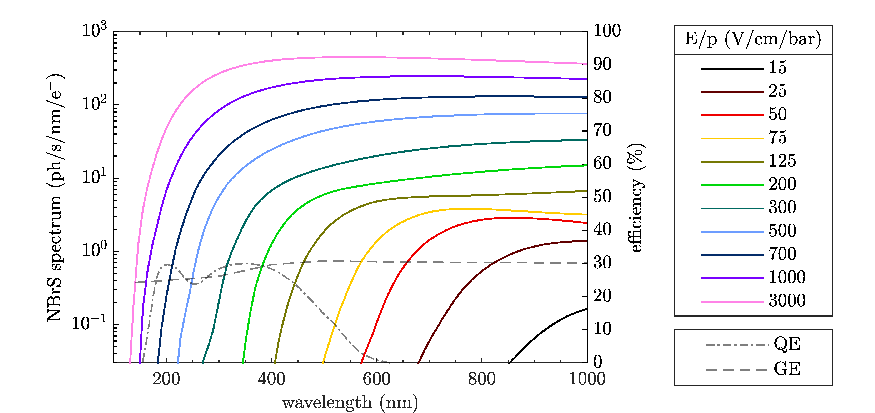
\includegraphics{Fig1.eps}
%\hfill
% "\includegraphics" is very powerful; the graphicx package is already loaded
\caption{\label{fig:spectrum}Computed NBrS emission rate as a function of wavelength for different electric field values. The quantum efficiency of the PMT used for the largest part of the measurements presented in this work is indicated by the dot-dashed line. The geometrical efficiency of the experimental setup, calculated with Geant4 (see a description later in the text), is indicated by the dashed line.}
\end{figure*}


\section{\label{sec:setup}Experimental setup and methodology}
\subsection{\label{subsec:NEW}The NEXT-White detector}

The NEXT collaboration seeks to discover the neutrinoless double beta ($0\nu\beta\beta$) decay of $^{136}$Xe using a high-pressure xenon gas time projection chamber with EL amplification \cite{a}. The unambiguous observation of $0\nu\beta\beta$ decay would prove lepton number violation and the Majorana nature of the neutrino. Xenon has no other long-lived radioactive isotopes that are expected to produce backgrounds to the double beta decay of $^{136}$Xe. The $^{136}$Xe $Q_{\beta\beta}$-value is relatively high ($\sim 2.5$ MeV \cite{b}) and the half-life of the $2\nu\beta\beta$ mode is in excess of 10$^{21}$ years \cite{c,d}. Therefore, $^{136}$Xe is an attractive isotope for $0\nu\beta\beta$ search as far as background is concerned.


\begin{figure*}[t]
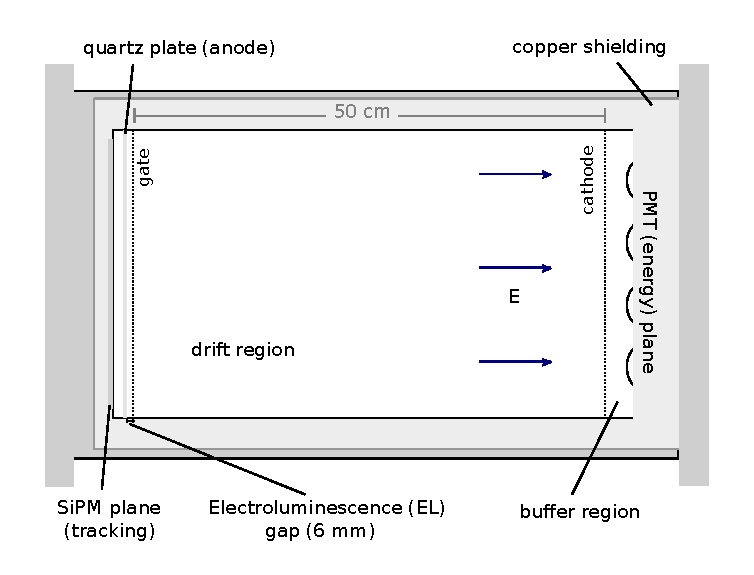
\includegraphics{Fig2.eps}
\caption{\label{fig:NEW_TPC}Schematic of the EL-based TPC developed by the NEXT collaboration for double-beta decay searches in $^{136}$Xe, adapted from \cite{46}.}
\end{figure*}


At present, NEXT is operating the largest HPXe optical-TPC, which is currently taking data at the Laboratorio Subterráneo de Canfranc (LSC) in the Spanish Pyrenees. The NEXT-White TPC (figure~\ref{fig:NEW_TPC}) is the first radiopure implementation of the NEXT TPC, and deploys $\sim 5$ kg of xenon in an active cylindrical volume of $\sim 53$ cm of length and $\sim 40$~cm in diameter, at a pressure of 10~bar. The energy measurement is provided by twelve Hamamatsu R11410-10 photomultiplier tubes (PMTs), having 31\% area coverage and placed 130 mm from a transparent wire mesh cathode, which is held at negative high voltage. A 2D-array (10-mm pitch) of 1792 SensL C-Series, 1-mm$^{2}$ silicon photomultipliers (SiPMs), placed few mm behind the electroluminescence (EL) gap, is used for particle track reconstruction. The EL gap is $\sim6$~mm thick and is defined by a stainless steel mesh and a grounded quartz plate coated with indium tin oxide (ITO) and TPB (tetraphenyl butadiene) thin films. An electric field is established in the drift region defined by the cathode and the gate mesh, while the electric field in the EL region is defined by the mesh voltage.

Charged particles deposit energy in the conversion (drift) region, the sensitive volume, producing a track of ionised and excited xenon atoms. The VUV scintillation resulting from the de-excitation processes and from electron/ion recombination, called the primary scintillation or S1 signal, provides the $t_0$ signal of the event, i.e. the start-of-event time-stamp. The ionisation electrons are guided towards the EL region by the drift field, whose value, around 40 V/cm/bar, is well below the xenon excitation threshold. In the EL region, under the influence of an electric field with an intensity between the gas excitation and the gas ionisation thresholds, each electron attains from the electric field enough kinetic energy to excite but not ionise the xenon atoms, by electron impact. In the de-excitation processes  a large amount of secondary scintillation (electroluminescence) is released, the S2 signal, without charge avalanche formation. The ($x,y$) positions of the electrons arriving at the EL region are determined by reading out the EL in the SiPM readout plane; the difference in time between the primary and the EL scintillation defines the $z$-position at which the ionisation event took place. These parameters can be conveniently used for fiducialising events that occur close to the chamber boundaries and that are, thus, likely to be from radiogenic backgrounds.

The TPC is connected to a gas system through which the gaseous xenon is continuously purified via a hot getter (MonoTorr PS4-MT50-R from SAES). The TPC active volume is shielded by a 60~mm thick ultra-pure inner copper shell, and the sensor planes are mounted on pure copper plates of 120~mm in thickness. The sensor planes and the active volume are enclosed in a pressure vessel constructed out of titanium-stabilized stainless steel alloy 316Ti. To reduce the background rate, the TPC is mounted inside a lead castle on a seismic platform in Hall A of LSC. The inner volume of the castle is flushed with radon-free air, with a $^{222}$Rn content 4–5 orders of magnitude lower compared to the LSC Hall A air \cite{e}, from a radon abatement system by ATEKO A.S. The experimental setup is similar to that of the preceding study \cite{f} and a comprehensive description of NEXT-White can be found in \cite{41}. 

The amplification of primary ionisation signals through EL results in both higher signal-to-noise ratio \cite{h,i}, due to the additional gain of the photosensor, and lower statistical fluctuations when compared to charge avalanche multiplication \cite{43}. The NEW TPC has demonstrated to attain energy resolution values below 1\%-FWHM \cite{46} at the xenon $Q_{\beta\beta}$, while the best energy resolution achieved in a smaller (1 kg) prototype based on charge avalanche amplification extrapolates to 3\%-FWHM \cite{L}. In addition, EL readout through photosensors, electrically and mechanically decouples the amplification region from the readout, rendering the system more immune to electronic noise, radiofrequency pickup and high voltage issues. When compared to LXe-based TPCs, HPXe TPCs achieve better energy resolution and allow for an efficient discrimination of the rare event through its topological signature based on track topology analysis with the determination of Bragg peaks at the ends \cite{L,m,n,6}. 

The energy (PMT) plane is used to trigger the detector, resorting to either the S1 or S2 scintillation signal. Individual waveforms obtained in the energy plane (summed over all PMTs), e.g. figure~\ref{fig:NEW_waveform}, are selected and classified as either `S1-like' or `S2-like'. Events with a single identified S1 are selected and the S2 peaks are divided into slices of 2-$\mu$s in width. The energies, $\varepsilon$, of the reconstructed deposition points along the track ($x, y, z, \varepsilon$) are, then, multiplied by two correction factors: one accounting for the geometrical ($x, y$) dependence of the light collection over the EL plane, and another one accounting for losses due to the finite electron lifetime caused by attachment to impurities. This second factor depends on both the drift length ($z$-coordinate) and the location on the EL plane ($x, y$), since the electron lifetime also varies in ($x, y$) due to the non-uniform distribution of impurities. Continuous detector calibration and monitoring was carried out with a $^{83m}$Kr low-energy calibration source, ensuring high-quality and properly calibrated low-background data \cite{p}. 


\begin{figure*}[t]
\centering % \begin{center}/\end{center} takes some additional vertical space
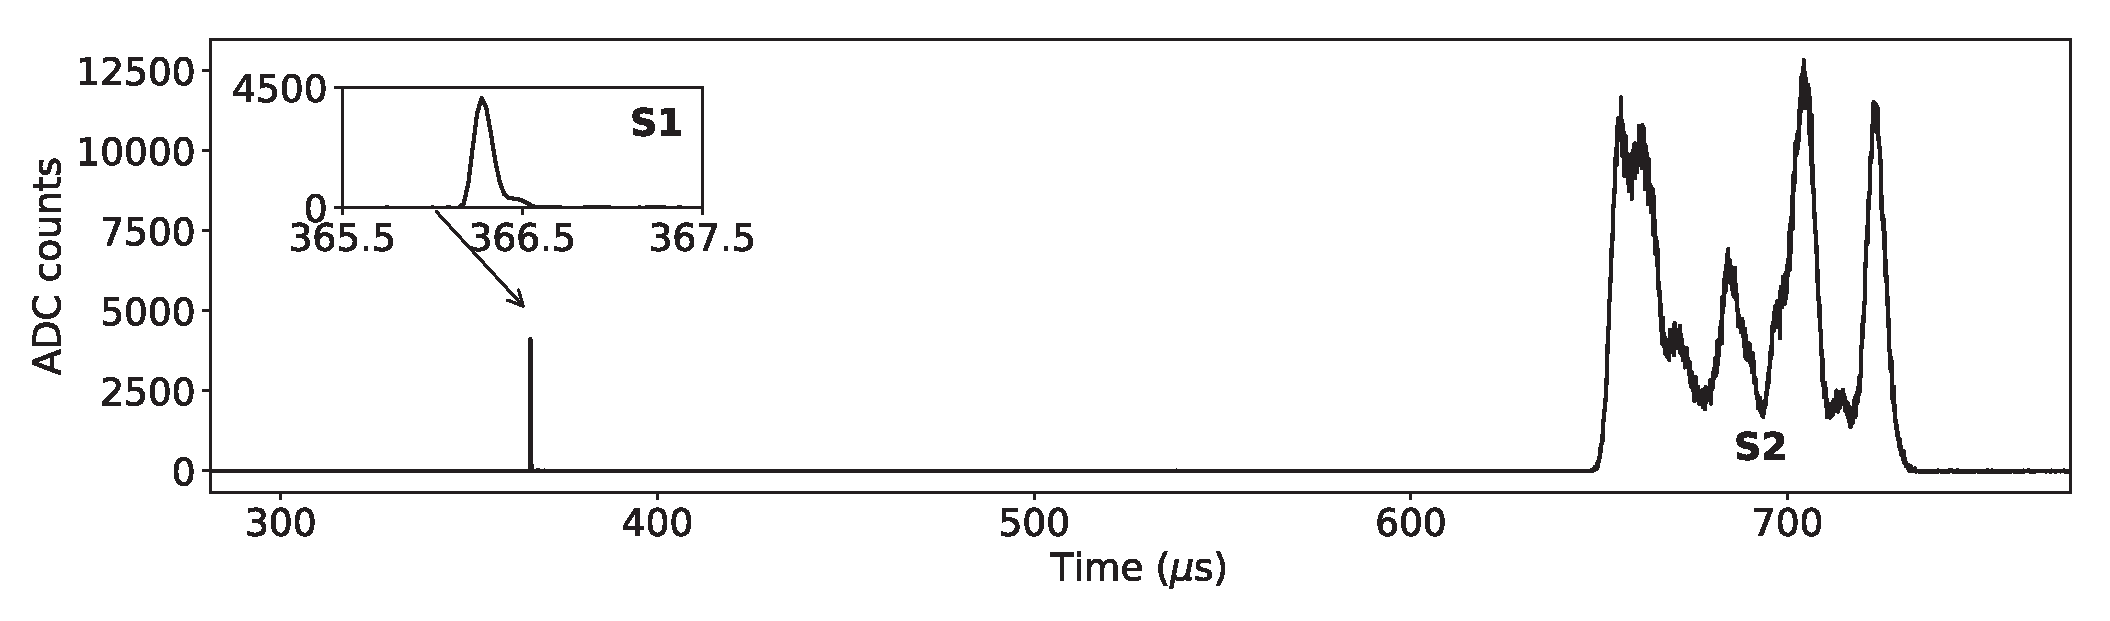
\includegraphics[width=\textwidth,height=\textheight,keepaspectratio]{Fig3.eps}
\caption{\label{fig:NEW_waveform}Typical waveform, summed over all PMTs, for an event due to $^{208}$Tl gamma (2.6~MeV) photoelectric absorption. The S1 and S2 signals are highlighted (adapted from \cite{46}).}
\end{figure*}

\begin{figure*}[tbp]
\centering
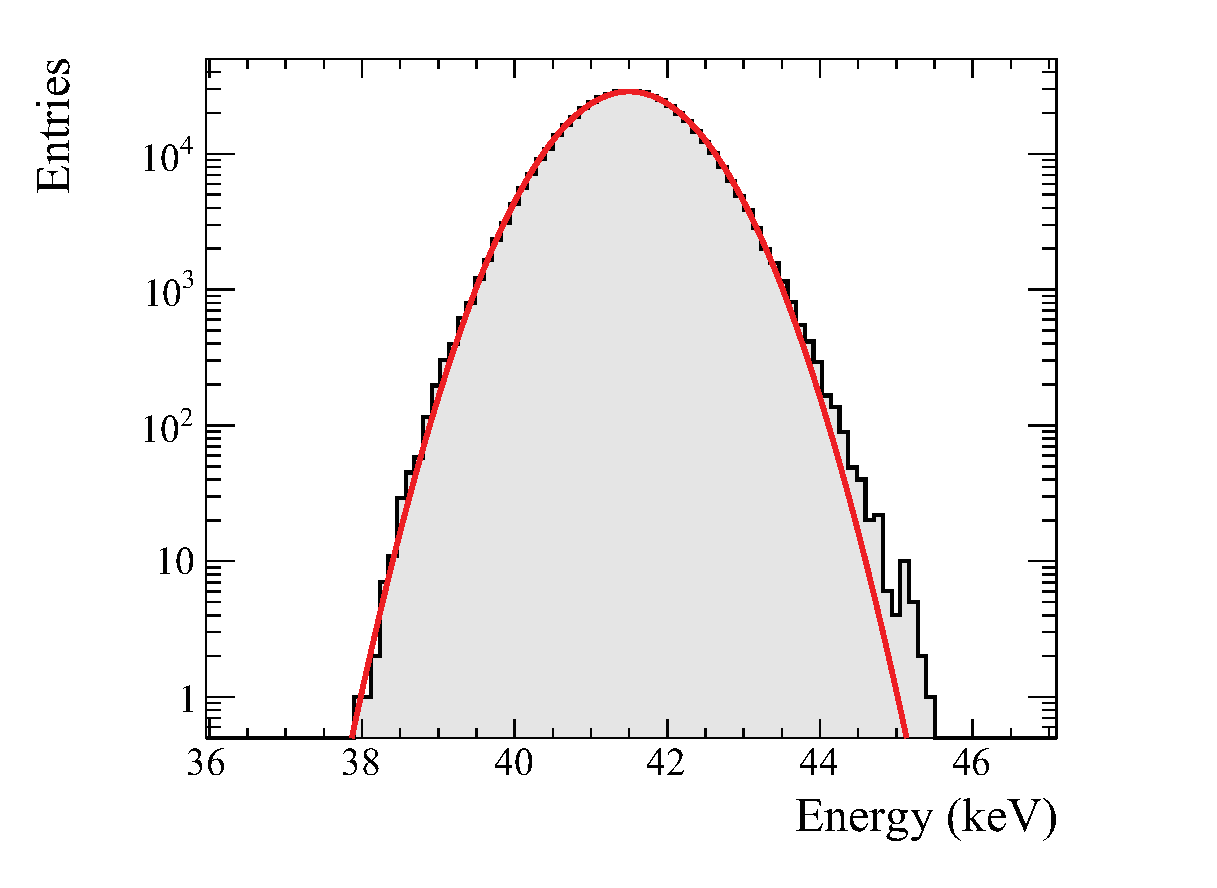
\includegraphics[width=0.495\textwidth]{Fig4a.eps}
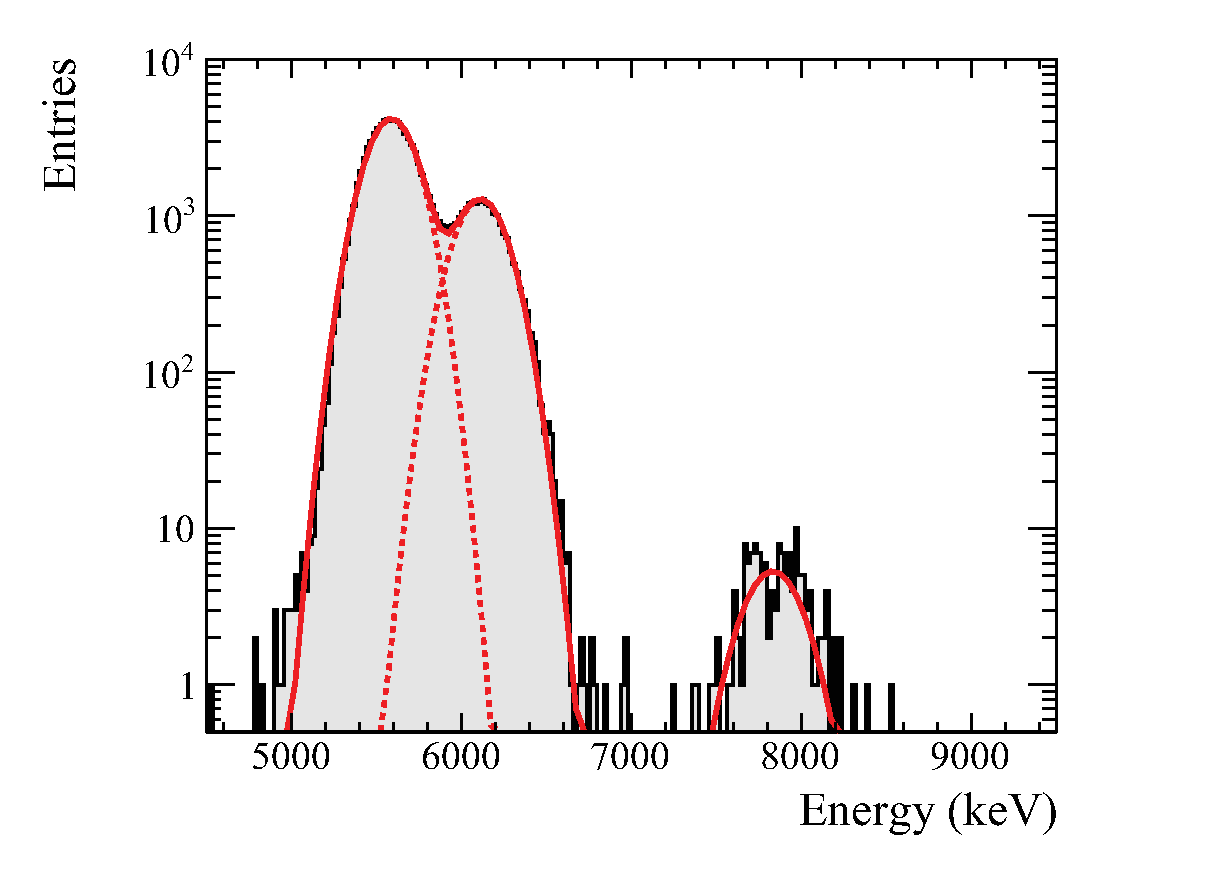
\includegraphics[width=0.495\textwidth]{Fig4b.eps}
\caption{Secondary scintillation (S2) spectra registered in the NEXT-White detector for $^{83\mathrm{m}}$Kr decays, 41.5 keV (left panel) and $^{222}$Rn (5.590 MeV), $^{218}$Po (6.112 MeV) and $^{214}$Po (7.834 MeV) alphas (right panel), obtained at 1.7~kV/cm/bar and 0.62~kV/cm/bar, in the EL region.} 
\label{fig:new_s2_spectra}
\end{figure*}

Compared to extended MeV-electron tracks, $^{83m}$Kr $\gamma$-rays as well as $\alpha$-particles produce nearly point-like energy deposits and the ($x, y, z$) corrections are straightforward. An example of the energy spectra reconstructed in both cases is shown in figure~\ref{fig:new_s2_spectra}. Circulating the xenon through a cold getter \cite{SAES} allowed us to have a source of radon-induced alphas in the whole fiducial volume, at a rate of several Hz. Therefore, alpha-rich runs, particularly at the beginning of a new experimental campaign, may be used to characterise the detector, similar to the regular calibration performed with $^{83m}$Kr. To this aim, a routine HV-scan was performed at 7~bar in the first runs of year 2017, at a much reduced EL-voltage in order not to saturate the PMTs. Further analysis, performed by studying the peak position of the alpha particles from the Rn progeny and that of $^{83m}$Kr $\gamma$-rays, revealed hints of an excess of scintillation below the EL-threshold, as shown in figure \ref{NEXTdata}.
Despite being a faint emission, it is very significant that alpha particles can still be identified in NEXT-White, for drift fields as low as 200~V/cm/bar, due to the presence of this sub-threshold emission. This observation motivated us to repeat the measurements under controlled conditions, with the idea to assign the nature of the phenomenon with as little ambiguity as possible, and exclude instrumental artifacts.



\begin{figure*}[tb]
\centering
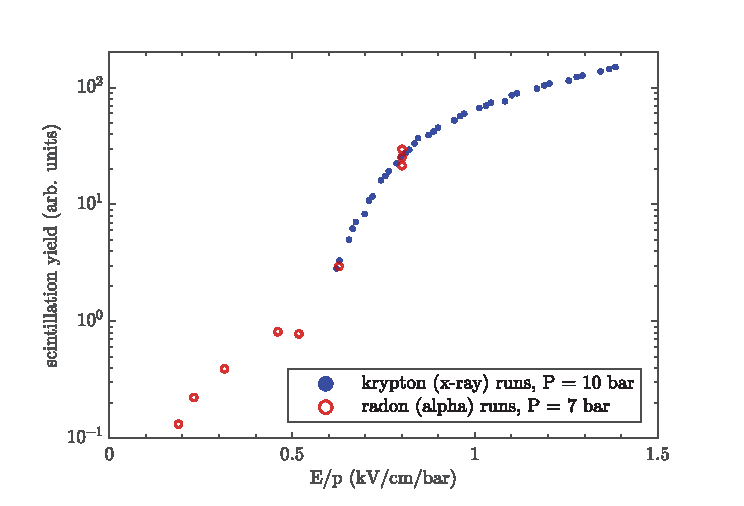
\includegraphics{Fig5.eps}
\hfill
\caption{\label{NEXTdata} Secondary scintillation (S2) measured for x-rays (closed circles) and $\alpha$-particles (open circles) with the NEW-TPC. No corrections for the wavelength-shifting effect of the TPB, light collection or quantum efficiency have been applied.}
\end{figure*}


\subsection{\label{subsec:dGPSC}The driftless GPSC}
For detailed studies on sub-threshold scintillation we employed a `driftless' GPSC that, unlike regular GPSCs used in \cite{43} for x-ray spectroscopy, does not feature a drift region (figure~\ref{fig:dGPSC}). Such a configuration is optimal for scintillation studies since it avoids any potential limitation due to electronegative impurities or charge recombination at typical drift fields, and does not require any optimisation of the primary electron transfer to the EL-region, usually done by means of a mesh.

\begin{figure*}[tbp]
\centering % \begin{center}/\end{center} takes some additional vertical space
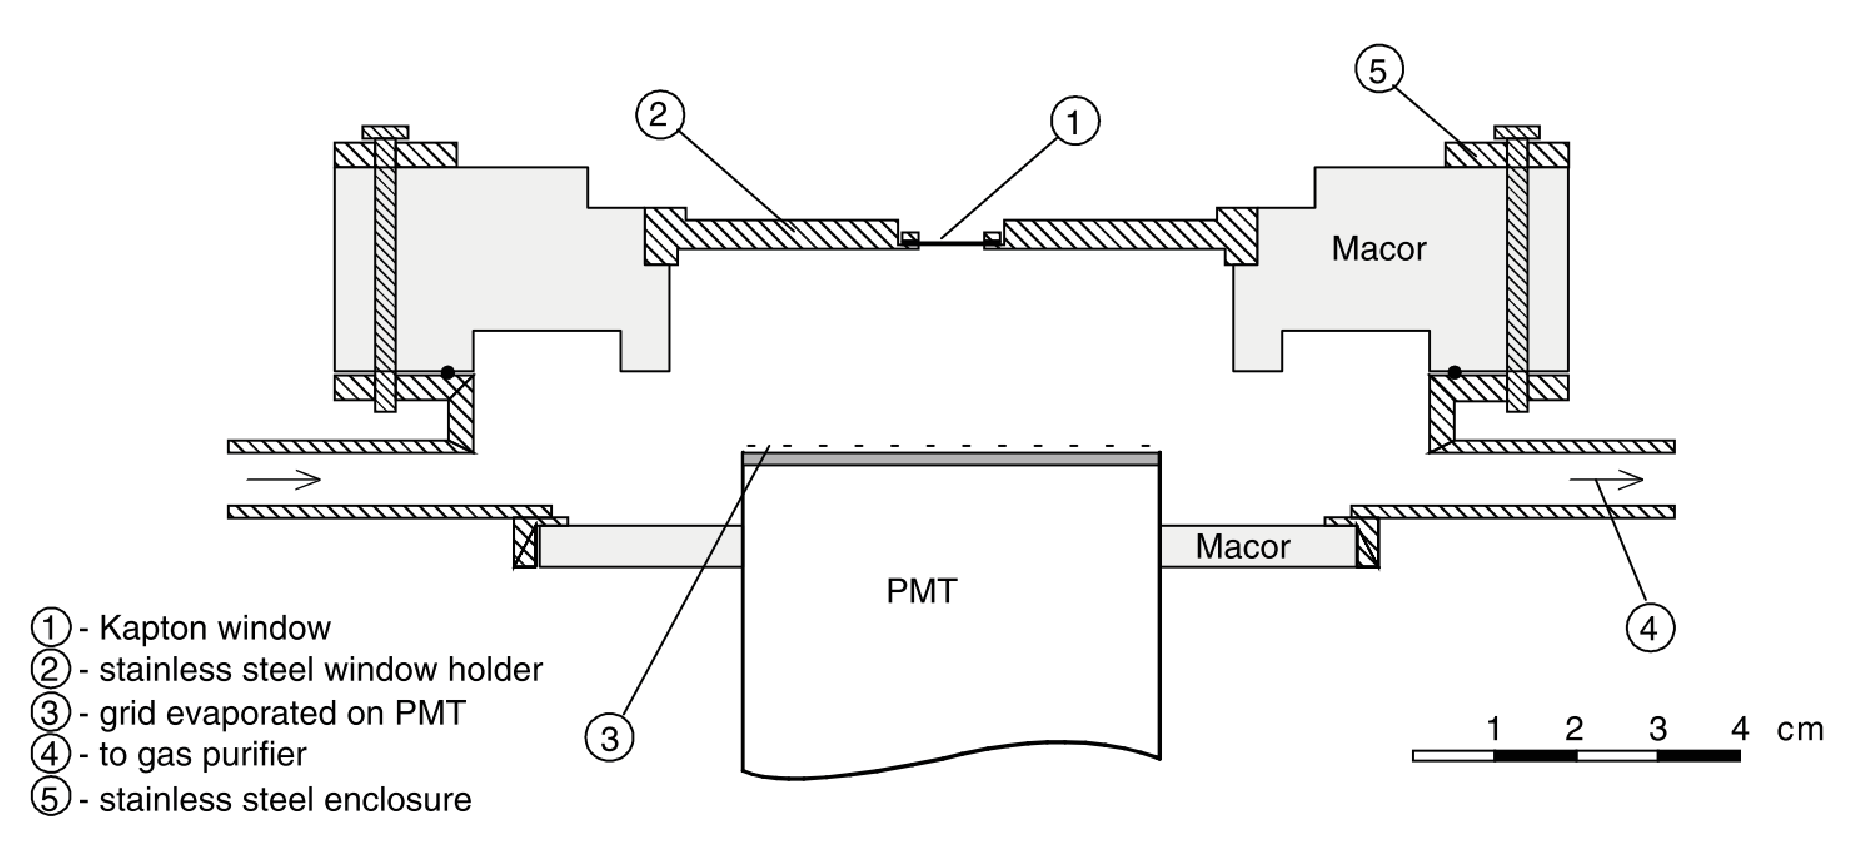
\includegraphics[width=\textwidth,height=\textheight,keepaspectratio]{Fig6.eps}
\caption{\label{fig:dGPSC}Schematic of the driftless GPSC used in this work, adapted from \cite{44}.}
\end{figure*}

In our chamber, the 2.45~cm-thick EL region is delimited by a Kapton window (8~mm in diameter, aluminised on the inner side, mounted on a stainless-steel holder), the cathode, and by the quartz window of our PMT, having on its outer surface a vacuum-evaporated chromium grid (100~$\mu$m thick  strips with 1000~$\mu$m spacing), the anode, electrically connected to the photocathode pin. Therefore, the electric field established between the anode and the cathode can be considered to be uniform along most of the region. The PMT (model EMI D676QB with 52~mm in diameter and a spectral sensitivity in the range of 155-625~nm, thereby avoiding the use of any wavelength-shifter) has been epoxied to a hollow Macor disc (about 10~cm in diameter), which has also been epoxied to the lower part of the detector, made of stainless steel and welded to the gas circulation tubing. The detector has been filled with pure Xe at a pressure of 1.24~bar (estimated temperature of about 300~K), with the gas being continuously purified through hot getters (SAES St‐707). This concept has been described in detail in previous studies \cite{42,44}.

A large number of primary electrons is required to reach an acceptable experimental sensitivity to the foreseen sub-threshold scintillation. Therefore, the detector was irradiated with alpha particles from a collimated \textsuperscript{241}Am source. A 5~$\mu$m Mylar film was placed between the source and the Kapton window to reduce the alpha particle penetration into the gas volume, so that the initial charge distribution is almost point-like and far away from the anode. The mean energy deposition and penetration depth were simulated using the software package `Stopping and Range of Ions in Matter' (SRIM) \cite{45}, yielding 1.7~MeV and 2.6~mm, respectively.   

The PMT output was connected directly to an oscilloscope (WaveRunner 610Zi from LeCroy), with a sampling rate up to 10~GS/s, using the 50~$\Omega$ DC coupling to match the cable impedance. Since the light emission studied in this work covers a wide range of intensities, the PMT bias voltage was adjusted between 650~V and 1400~V, to reach optimal signal-to-noise ratio, while avoiding PMT saturation. PMT gain calibration was performed with a pulsed LED, in order to correct results obtained at different PMT voltages. For convenience, PMT waveforms were acquired with a sampling time of $\sim$3.5~ns. Prior to data analysis, a background discrimination algorithm rejects events based on waveform duration, time offset and shape, as well as on baseline cleanliness.


\begin{figure*}[tbp]
\centering % \begin{center}/\end{center} takes some additional vertical space
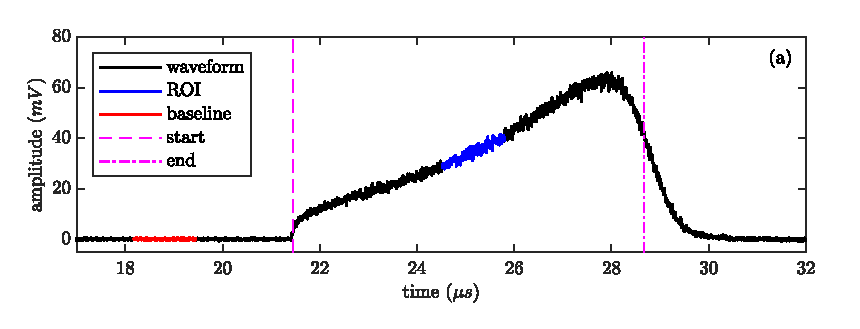
\includegraphics[]{Fig7a.eps}
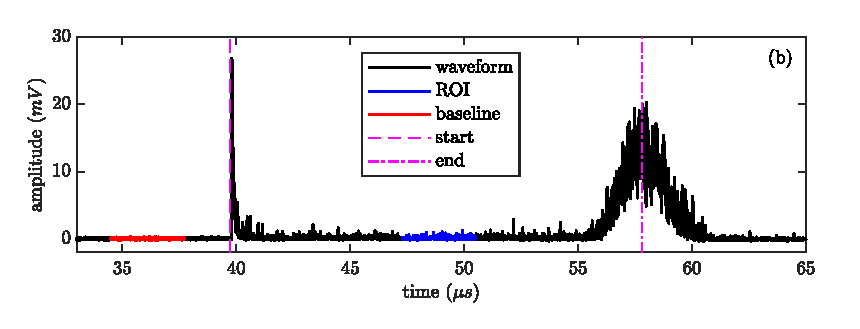
\includegraphics[]{Fig7b.eps}
\hfill
% "\includegraphics" is very powerful; the graphicx package is already loaded
\caption{\label{fig:waveforms}Typical driftless GPSC waveforms obtained for a high $E/p$ (1.5 kV/cm/bar) (a) and for a low $E/p$ (320 V/cm/bar) (b). The start and end of the events are represented by vertical lines. The regions considered to determine the NBrS and EL emissions, and the baseline offset, are also shown in blue and red, respectively.}
\end{figure*}

Figure~\ref{fig:waveforms} (a) depicts a typical waveform. The amplitude growth over time results from the increasing solid angle subtended by the PMT window as the electron cloud drifts towards the anode. However, when the reduced electric field is below the EL threshold, the PMT waveform reveals features that would go, otherwise, unnoticed as shown in figure~\ref{fig:waveforms} (b). The first short peak corresponds to the primary scintillation signal (S1) from the alpha particle interaction while the last, longer peak results from the secondary scintillation (S2) produced when the ionisation electrons are close to the anode strips, where the non-uniform electric field is above the EL threshold. In addition, many smaller and shorter peaks can be observed between the two major ones, a phenomenon that can be, unambiguously, assigned to single-photon emission during the drift of the ionisation electrons. 

\begin{figure}[tbp]
\centering % \begin{center}/\end{center} takes some additional vertical space
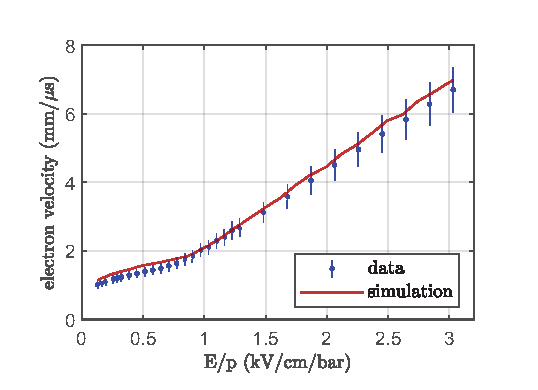
\includegraphics[scale=0.9]{Fig8.eps}
\hfill
\caption{\label{fig:vd}Electron drift velocity determined from the driftless GPSC waveforms as a function of reduced electric field, compared with the simulated curve obtained with Magboltz.}
\end{figure}

Our interpretation of the origin of the `start' and `end' features of the waveforms shown in figure~\ref{fig:waveforms} can be confirmed by comparison with the expected drift velocity in pure xenon. This was obtained, for each run, from both the distribution of waveform duration and the mean range (along the electric field direction) of the alpha particles (from SRIM). The start of event is given by the instant the waveform amplitude rises by 5 \% of its maximum height, while the end of event is defined as the instant the centre of the electron cloud reaches the anode. For low-field waveforms (figure~\ref{fig:waveforms}-bottom), that instant corresponds to the centroid of the (diffusion-dominated) S2 peak, while for high electric fields (figure~\ref{fig:waveforms}-top) it corresponds to the instant the amplitude falls to 65 \% of the waveform maximum. This last value was estimated by simulating the drift-diffusion of the electron cloud, considering the detector geometry and the PMT response function. Nonetheless, there is a transition between the two distinct waveform shapes when the electric field reaches values close to the EL threshold. In this case, the end of event is linearly interpolated between the waveform maximum and the 65 \% threshold. The electron drift velocity obtained through this procedure is depicted in figure~\ref{fig:vd} for several $E/p$ values, together with the simulated curve from Magboltz. The agreement between experimental and simulated data is acceptable, and the observed deviation is included as a contribution to the overall systematic uncertainty of the scintillation yield per unit path length.   


\begin{figure}[h!!!]
\centering % \begin{center}/\end{center} takes some additional vertical space
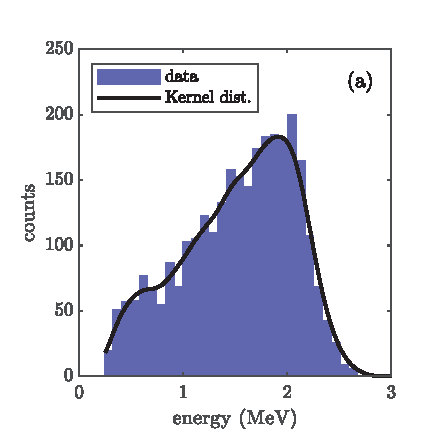
\includegraphics[]{Fig9a.eps}
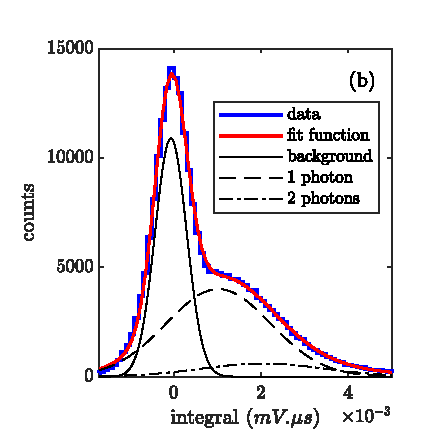
\includegraphics[]{Fig9b.eps}
\hfill
\caption{\label{fig:dist}(a) Typical energy spectrum of alpha particles in the GPSC detector taken for an E/p value of 1.5 kV/cm/bar, fitted to a Kernel distribution in order to estimate the peak energy. (b) Distribution of the integral of photon pulses, obtained for a low $E/p$ value (300~V/cm/bar), in the waveform ROI. It has been fitted to a sum of Gaussian distributions, accounting for the background, single, double, triple and quadruple photon detection, being the latter two not visible in the graph.}
\end{figure}

Due to the angular distribution of the alpha particles and the presence of the entrance window and degrading foil, a selection cut on the primary ionisation has to be applied. Figure~\ref{fig:dist} (a) shows the typical energy spectrum for alpha particles obtained from the histogram of waveform integrals. The lack of events at low energies results from the oscilloscope trigger threshold. A \textsuperscript{55}Fe radioactive source was used to calibrate the detector energy for a given $E/p$ value (2.9~kV/cm/bar). In this way, a peak energy of 1.9~MeV was measured for alpha particles, in good agreement with the SRIM~simulated value, 1.7~MeV. Since the shape of the energy spectrum was found not to depend significantly on $E/p$, the peak of the distribution was used to calibrate the remaining data sets acquired for each $E/p$ value. Indeed, the recombination of ion-electron pairs produced by the alpha particle interaction is expected to be negligible for the relatively high $E/p$ values studied in this work \cite{recombination}. Moreover, we did not find any significant change of the primary scintillation yield, which is anti-correlated with the number of ionisation electrons, within the studied $E/p$ range. To reduce the influence of the oscilloscope trigger threshold, a 1.6~MeV energy cut was applied to the data. Again, as before, the discrepancy between measurements and SRIM~simulation was included in the systematic uncertainty of the yield values.

Finally, in order to determine the scintillation yield, it is desirable to select a waveform region that is i) sufficiently delayed with respect to S1 to exclude the Xe de-excitation tail of the triplet state and any PMT after-pulsing, and ii) sufficiently ahead of the diffusion-dominated anode signal. Hence, a short region of interest (ROI) was defined midway between the time the event starts and the time it ends, accounting for the photons emitted when the electron cloud is between 0.9 and 1.3 cm away from the anode. An important side benefit of this procedure is the simplification of the geometrical corrections needed for comparison with simulation.
Then, the average value of the waveforms' integrals performed in the 4~mm ROI (in blue in figure~\ref{fig:waveforms}) was computed, subtracting the integrated baseline prior to the event (in red in figure~\ref{fig:waveforms}). The yield estimated in this way can be calibrated to an absolute number of detected photons per unit path length, after considering the integral signal produced by single photons, as determined before-hand for ambient photons.

For low electric fields, the aforementioned technique loses precision as the NBrS emission is at the level of the baseline fluctuations, requiring large statistics. However, since the NBrS signal consists mostly of individual photon peaks (see figure~\ref{fig:waveforms}-bottom), single-photon counting techniques may be applied. To reduce the effect of low~frequency baseline fluctuations, the ROI is processed in a software high~pass filter. Afterwards, every peak found in this region, above a given threshold, is integrated. Figure~\ref{fig:dist} (b) shows an example of the distribution of the integrals of these peaks for an $E/p$ value of 300~V/cm/bar. Finally, a suitable fit function is used to estimate the total number of detected photons, which is, subsequently, normalised to the number of events. This function, also shown in figure~\ref{fig:dist} (b), consists of a sum of five Gaussian functions, the first one accounting for the high~frequency noise of the signal, with area, centroid and sigma being left as free parameters, while the subsequent ones account for single, double, triple and quadruple photon detection. Their centroids ($c$) follow the scalings $1{c}$, $2{c}$, $3{c}$ and $4{c}$, with standard deviations ($\sigma$) following $\sqrt{1}\sigma$, $\sqrt{2}\sigma$, $\sqrt{3}\sigma$ and $\sqrt{4}\sigma$, respectively, being the areas related through Poisson statistics. The mean value of the Poisson distribution, the centroid and the standard deviation of the single-photon Gaussian are left as free parameters.  
Results from both photon-counting and integral method are presented in the next section.

\section{\label{sec:results}Experimental results and discussion}

The xenon secondary scintillation yield as a function of $E/p$ measured over 5 orders of magnitude, is shown in figure~\ref{fig:nBr} (a table with the numerical data can be found in the appendix \ref{sec:values}). The yield has been normalised to the gas pressure, path length and number of ionisation electrons. The latter was obtained from the average energy deposited by alpha particles in the gas, after performing the aforementioned 1.6~MeV cut and assuming a $w$-value of 21.9~eV, i.e., the mean energy required to produce an electron-ion pair, \cite{carmo} and references therein. Two data sets are shown, one of them obtained using the waveform averages (blue markers) and the other one, for low $E/p$ values, obtained by photon counting (red markers), as discussed in section \ref{subsec:dGPSC}. For $E/p$ values below 400~V/cm/bar, the scintillation in the ROI is sufficiently low to enable the use of the more precise photon counting method. When $E/p$ is around 350~V/cm/bar, our standard analysis based on the waveform average is still precise, allowing for a direct comparison between both methods. 
The good agreement observed in this region shows the accuracy of the photon counting method, which becomes more reliable at lower electric fields.
The error bars represent the 68\% confidence level regions, comprising both systematic and statistic uncertainties associated to the analysis methodology and instrumental limitations (a list of the different uncertainty sources can be found in the appendix \ref{sec:values}). An inflection point can be observed in the experimental data at low $E/p$ values, below the EL threshold, suggesting the existence of a different emission mechanism in that region. This emission, despite being weak, is still measurable for about two orders of magnitude below the intercept point of the two contributions and is, ultimately, limited by the QE of the PMT.

\begin{figure*}[t]
\centering % \begin{center}/\end{center} takes some additional vertical space
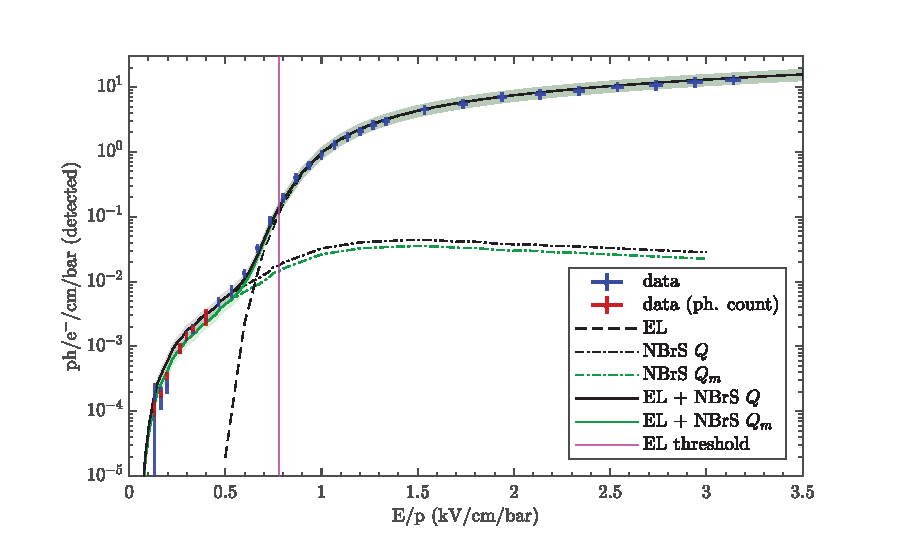
\includegraphics{Fig10.eps}
\hfill
\caption{\label{fig:nBr}Number of detected photons obtained with the driftless GPSC as a function of reduced electric field, being the value normalised according to the gas pressure, drift path and number of primary ionisation electrons. At low electric fields, the experimental results obtained with the photon counting method are also shown (points in red). Error bars present the 68~\% confidence levels of the experimental data. The EL threshold is also presented; it is commonly defined as the intercept of a line, fitted to the EL yield as a function of $E/p$, with the $x$-axis; only high $E/p$ values where this relationship is approximately linear are used. Simulated curves are superimposed to the data, being the NBrS yield obtained assuming proportionality with either $Q$ or $Q_m$. Coloured bands present the systematic error associated to the simulation curves, dominated by the 20~\% uncertainty estimated for the detection efficiency.}
\end{figure*}

In order to better disentangle the different contributions to the measured scintillation, we proceeded in the following way: the emission at high $E/p$ values (assumed to be excimer-based, EL emission) was simulated with the microscopic package introduced in \cite{31}, while the emission at low $E/p$ values (assumed to be NBrS) was determined by resorting to the new features of the recently developed python-version of the Magboltz code \cite{Pyboltz}, allowing for an easy implementation of the simple theoretical framework described in section \ref{sec:nBr}. The final calculation of the number of detected photons requires taking into account the wavelength-dependent PMT quantum efficiency (QE($\lambda$)) and geometrical efficiency (GE($\lambda$)), shown in figure~\ref{fig:spectrum}. The QE was obtained from the manufacturer and GE from Geant4 simulation \cite{geant4}, figure~\ref{fig:QEGE}-left. As a result of the dependence of the NBrS emission spectrum on the reduced electric field, the detection efficiency ($\mathcal{D}$) becomes field-dependent. Its value, averaged over the range of 120-1000~nm ($\mathcal{D}=<$QE$\times$GE$>_\lambda$), is shown in figure~\ref{fig:QEGE}-right. A 20\% uncertainty was assigned to $\mathcal{D}$, dominated by the assumptions on the reflectivity of the materials.

\begin{figure*}[tbp]
\centering % \begin{center}/\end{center} takes some additional vertical space
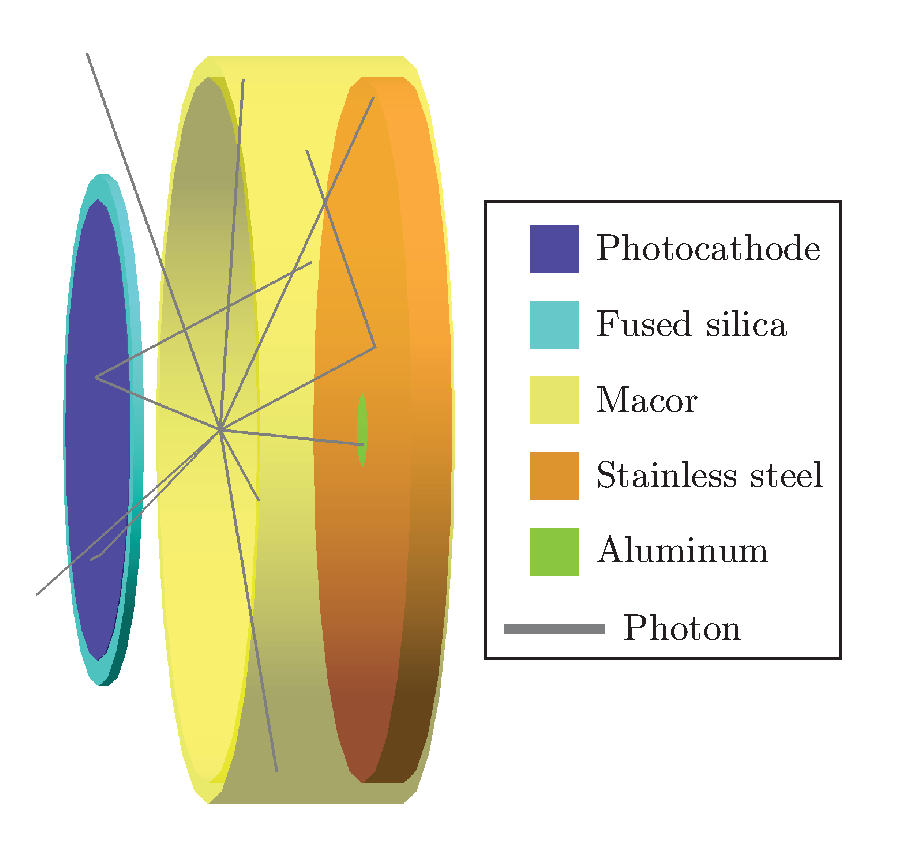
\includegraphics[width=7.4cm,height=7cm,keepaspectratio]{Fig11a.eps}
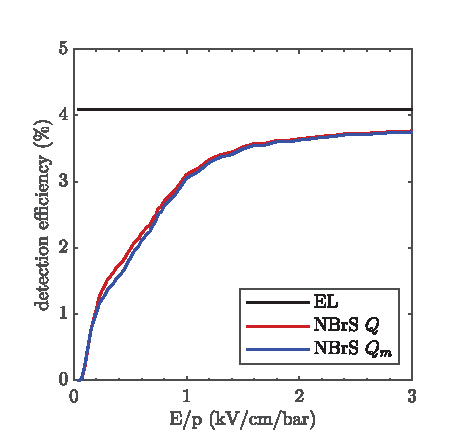
\includegraphics[]{Fig11b.eps}
\hfill
\caption{\label{fig:QEGE}Left: geometry used in Geant4 for the calculation of the light collection efficiency of the driftless GPSC, including the most relevant detector materials. The transparency of the anode grid ($\mathcal{T}=81$~\%) was included as a multiplication factor over the simulated value. On the right, the overall detection efficiency averaged over the 120-1000 nm range ($\mathcal{D}=<$QE$\times$GE$>_\lambda$), is shown as a function of reduced electric field, considering both the EL and NBrS spectra. A dependence with either $Q$ or $Q_m$ has been assumed in expression \ref{nBr_eq4}. A 20~\% uncertainty was estimated for $\mathcal{D}$, being dominated by the uncertainty in GE, and obtained by varying the optical parameters in the simulation (macor, stainless steel and aluminum reflectivities).}
\end{figure*}

The excellent agreement data-simulation makes a very compelling case for NBrS as being responsible for the observed sub-threshold emission. The systematic uncertainty on the simulated light yield in figure~\ref{fig:nBr} is expected to be dominated by the estimated 20\% uncertainty on the detection efficiency, both for its EL and NBrS components, and for all $E/p$ values. As a consequence, the observed scintillation excess over EL scintillation-only expectations at low $E/p$ values is extremely significant, providing very strong evidence for this additional scintillation mechanism. Moreover, we can exclude this emission from being EL by demonstrating its different radiative nature when compared to the excimer-nature of EL. This comparison can be easily highlighted by the addition of a controlled trace-amount of molecular additive, chosen to be C$_{2}$H$_{6}$, in this case, at a concentration of $0.12\%$. As in previous work \cite{42,44}, the concentration was monitored during data taking with a Residual Gas Analyser and a sampling system, in order to eliminate effects related to getter-absorption of the additive. The two experimental methods (integral and photon-counting) are statistically combined and shown in figure~\ref{fig:mix}-left.
The shift of the Xe-C$_{2}$H$_{6}$ data series towards higher $E/p$ values is due to electron cooling, enhanced through inelastic transfers to vibrational and rotational states of the molecular additive \cite{42,32,44}. Thus, the electric field needs to be higher to provide the electrons with the energy lost to the molecules. According to \cite{CH_thesis}, the electron cooling effect can be compensated by a suitable shift of the reduced electric field (corresponding to 100 V/cm/bar, in this case), as shown in figure~\ref{fig:mix}-right. After accounting for electron cooling in this approximate way, we find that the impact of the additive on the low $E/p$ scintillation is negligible, and the NBrS emission can be fully recovered, in contrast to the situation for high $E/p$ values, where the EL suffers permanent losses due to the quenching of the excited xenon triplet states by the molecular additive. 
The impact of C$_{2}$H$_{6}$ on NBrS and EL emissions was also simulated, as shown in figure~\ref{fig:mix}-left. First of all, it is noticeable how the shift of the NBrS contribution, due to electron cooling, is correctly reproduced. Concerning the EL-contribution, on the other hand, the quenching probability $P_Q$ was left as a free parameter, with a best description of data found at a scintillation probability of $P_{scin}= 1- P_Q =55\%$, a value that acts as a global factor multiplying the EL contribution for all fields. An independent estimate, considering the simple model in eq. (14) of \cite{32}, yields $P_{scin}=37\%$, if introducing the quenching rate of the first excited state of Xe in the presence of C$_2$H$_6$, as measured by Setser and coworkers \cite{Setser}.

In general, and despite the good agreement data-simulation when including the NBrS expression given in eq. \ref{nBr_eq4}, our data shows, at low fields, a clear preference towards using $Q_m$ in that formula, shifting to $Q$ at intermediate fields, before excimer-driven EL takes over. A more accurate description of this phenomenon would certainly benefit from additional theoretical efforts.

\begin{figure*}[tbp]
\centering % \begin{center}/\end{center} takes some additional vertical space
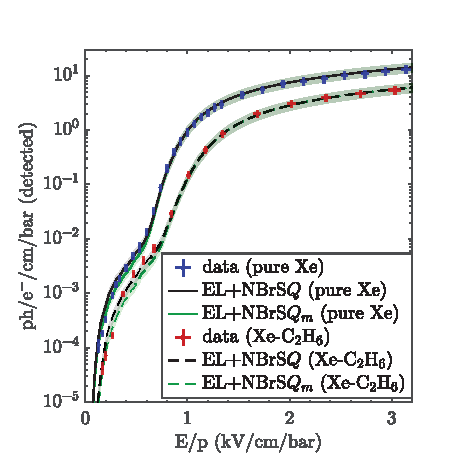
\includegraphics[]{Fig12a.eps}
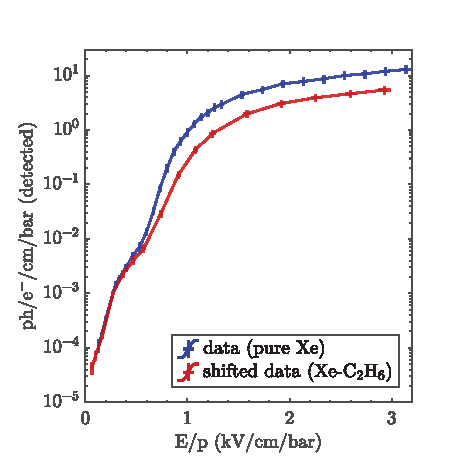
\includegraphics[]{Fig12b.eps}
\hfill
\caption{\label{fig:mix}On the left, the number of detected photons (68 \% confidence level depicted as error bars) obtained experimentally with pure Xe and a Xe-C$_{2}$H$_{6}$ admixture (with a 0.12 \% C$_{2}$H$_{6}$ concentration), together with the respective simulated curves (systematic error depicted as coloured bands). The experimental results provided by the two analysis methods for low electric fields have been statistically combined. On the right, the Xe-C$_{2}$H$_{6}$ curve was shifted to the left by 100 V/cm/bar, illustrating the different nature of the low-$E/p$ emission since it is not quenched, unlike the EL (excimer-based) contribution.}
\end{figure*}

\begin{figure*}[tbp]%[h!!!]
\centering % \begin{center}/\end{center} takes some additional vertical space
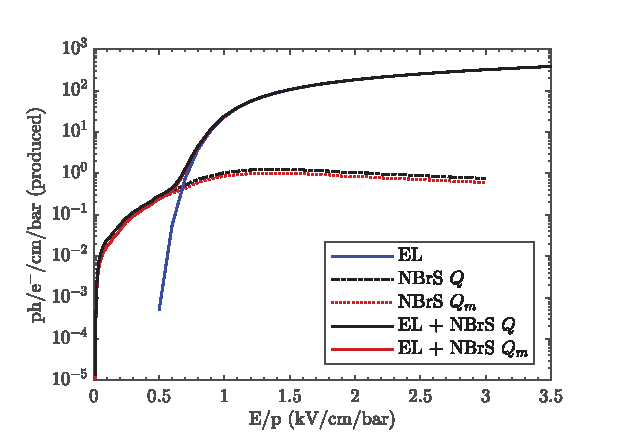
\includegraphics[]{Fig13a.eps}
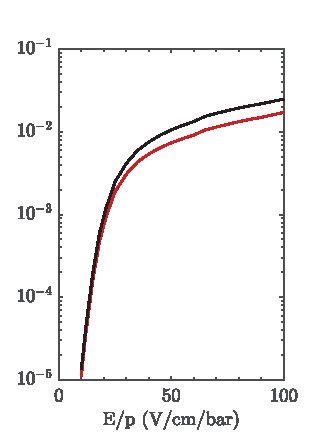
\includegraphics[]{Fig13b.eps}
\caption{\label{fig:produced}Simulated secondary scintillation yield in the range of 120-1000~nm as a function of $E/p$. A dependence with either $Q$ or $Q_m$ has been assumed in expression \ref{nBr_eq4}. The individual contributions from EL and NBrS are shown ($T=300$~K). A detail of the 0-100 V/cm/bar region is shown on the right side.}
\end{figure*}

From figure~\ref{fig:nBr}, one can see that, for nominal EL-field values above 1 kV/cm/bar, the NBrS contribution to the xenon secondary scintillation is less than 1\%, insufficient to modify, in a perceptible manner, the calorimetric response of xenon TPCs. Moreover, for the operating conditions of the NEXT-White TPC, the drift field of 40 V/cm/bar renders the PMTs insensitive to the NBrS emission during electron drift, figure~\ref{fig:spectrum}, due to their lack of sensitivity above 600 nm. The SiPM plane, despite being sensitive in this range, lacks coverage, being the NBrS emission insufficient, as well, to be significantly perceptible. On the other hand, in the NEXT-White TPC, in the buffer region between the cathode and the (grounded) PMT plane, the electric field intensity is of the order of some 100’s of V/cm/bar, which is sufficient to produce NBrS scintillation detectable by the PMT plane. These signals have been observed in the NEXT-White TPC, similar to single photo-electron signals during the corresponding primary electron drift time in this region. A similar situation is likely to occur in the buffer region, between the anode and the top PMT plane electrode, in the gas phase of double phase TPCs used for direct dark matter searches.

Finally, in order to address the interest of NBrS, figure~\ref{fig:produced} presents the simulated scintillation yield, for pure xenon, integrated in the region of 120-1000~nm. One may conclude that, for electric fields as low as 50~V/cm/bar, and if resorting to a sensor with sensitivity up to around 1000~nm (e.g. the latest Hamamatsu SiPMs present a sensitivity that extends to nearly 1000 nm, with a PDE around 5\% at 900 nm \cite{SiPMs}), the observable scintillation yields would still be at the levels reported here. This field is about $40$ times lower than those conventionally used in EL amplification and almost $1000$ times lower than those typically used in avalanche-based amplification. In opposition to EL, NBrS is broadband and, as shown in this work, it does not undergo quenching in the presence of additives. Since, at low electron energies, NBrS is related to the electron-atom elastic cross section, it can be expected to be present in any gas. 
In the NEXT-White TPC, without any optimisation, NBrS produces measurable signals from $\alpha$-particles down to 200~V/cm/bar and, plausibly, down to 50~V/cm/bar if the QE of the sensors extends up to 1000~nm. 
For reduced electric fields below 10~V/cm/bar, the electron energy distribution becomes thermal, shifting the wavelength cutoff up to around 4000~nm, thus making it virtually undetectable in a TPC with the existing technology. This is likely the case for electrons drifting in LXe TPCs \cite{XENON, LZ, EXO}, where a direct application of density-scaling would situate the reduced field at values corresponding to 1~V/cm/bar in figure \ref{fig:produced}. The estimate comes from assuming a factor of $\times 500$ higher density for liquid xenon than for gaseous xenon at NTP conditions, and a typical drift field around 500~V/cm in the former case. Therefore, our results suggest a negligible NBrS scintillation emission stemming from drifting electrons in the liquid phase in contemporary LXe TPCs, if assuming that a density-scaled gas phase emission is approximately valid for describing the situation, even when considering a detectable range of 120-1000 nm. The drifting electron cloud with energies very close to thermal energy, which is anticipated for typical drift fields of the order of 500 V/cm, would yield an emission outside this window and deep into the infrared range. On the other hand, in the buffer region in LXe, between the cathode and the bottom PMT plane electrode, or in any other region in the LXe, NBrS photon emission in the sensitivity range of the PMTs will likely occur if the electric field is set above few tens of kV/cm (e.g., in the LZ TPC it is foreseen that the electric field intensity in the LXe may reach values almost as high as 35 kV/cm \cite {LZ}).


The situation, however, is much more interesting concerning the prospects for secondary scintillation. Conservatively assuming an electric field of 100~kV/cm (a factor of $4$ below the breakdown field reported in \cite{EB}), the application of density scaling would lead to an NBrS yield of 50~ph/e$^{-}$/cm. Given the unusual characteristics and faint nature of this phenomenon, it is conceivable that it might have gone unnoticed in previous experiments or, else, misinterpreted, as recently referred in \cite{nBrLast}. Because of the utmost importance of obtaining secondary scintillation directly from the liquid, and with all reservations due to the absence of a first-principle simulation of NBrS in those conditions, it seems to these authors that this new R\&D line presents a strong path to be pursued with determination in the upcoming future. 

\section{\label{sec:conclusions}Conclusions}

In this paper we present the first unambiguous identification of NBrS luminescence in xenon, supported by a predictive theoretical model of this light-emission process.
We present compelling evidence of radiation being emitted by low-energy ionisation electrons in the dipole field of xenon atoms at electric fields of interest for TPCs used in rare event searches: We have shown its presence in the NEXT-White TPC, at present the largest optical HPXe-TPC in operation, we performed detailed measurements in a dedicated setup and implemented a robust theoretical model for NBrS, which describes the data very well. NBrS emission is intrinsically broadband and, as confirmed by our measurements, immune to quenching mechanisms, unlike conventional excimer-based electroluminescence emission. Since it does not create additional electrons nor ions, NBrS is expected to be free from ion feedback or ageing issues. This mechanism produces scintillation levels that are detectable with standard sensors. Hence, it is seemingly of relevance in a range of reduced electric field values, extending from those employed for secondary scintillation ($\mathcal{O}(1 {kV/cm/bar})$) to typical drift fields of $\mathcal{O}(100 {V/cm/bar})$, arguably down to the thermal limit (around $E/p=10$~V/cm/bar in pure xenon at room temperature). 

Nevertheless, for nominal EL-field values above 1 kV/cm/bar, the NBrS contribution to the secondary scintillation is less than 1\%,  insufficient to modify, in a perceptible manner, the calorimetric response of xenon TPCs. 
Similarly, for typical drift fields below 50 V/cm/bar, the NBrS emission falls below the sensitivity range of conventional PMTs. On the other hand, it will be perceptible in the TPC buffer regions in the gas phase, between the high voltage electrode and the ground electrodes shielding the PMT planes. For LXe, NBrS emission in the sensitivity range of the PMTs will only likely happen in regions where the electric field value is above few tens of kV/cm.

At present, NBrS photon emission in Xe TPCs may be seen as a nuisance. Even it that would be the only implications, it would still require a detailed understanding, in particular in the era of dark matter (and coherent neutrino scattering) experiments which aim to detect single-photons associated to the ionisation produced by nuclear recoils of very small energy. In such a regime, the single photoelectron emission observed in the NEXT-White detector and other devices and most likely associated to NBrS, could eventually mask the tiny signals associated to new physics. A clear corollary or our work is that the ample community of neutrino and dark matter experiments based in xenon cannot longer ignore NBrS. 

Conversely, a deep understanding of the effect may  have implications in the design of future TPCs, namely avoiding hot spots in the LXe and avoiding high electric fields in the buffer regions, effects, which, up to now, have not been considered with special attention.  

Last but not least, the possibility of implementing a scintillation mechanism such as NBrS directly in the LXe opens up intriguing possibilities towards the development of single-phase LXe TPCs based on secondary scintillation amplification of the ionisation signal, avoiding the prohibitively high electric fields required by EL production in LXe, which could, eventually limit the scalability of future detectors.  

As an example, we would like to mention the possibility to produce ionisation signal amplification through secondary scintillation (e.g., NBrS), which could be achieved directly in the liquid, using hole-type structures capable of sustaining electric fields around 100 kV/cm, over cm-long distances. Such technique could revolutionise the design of future neutrino and dark matter experiments.

\begin{acknowledgments}
The NEXT Collaboration acknowledges support from the following agencies and institutions: the European Research Council (ERC) under the Advanced Grant 339787-NEXT; the European Union’s Framework Programme for Research and Innovation Horizon 2020 (2014–2020) under the Grant Agreements No. 674896, 690575 and 740055; the Ministerio de Econom\'ia y Competitividad and the Ministerio de Ciencia, Innovaci\'on y Universidades of Spain under grants FIS2014-53371-C04, RTI2018-095979, the Severo Ochoa Program grants SEV-2014-0398 and CEX2018-000867-S, and the Mar\'ia de Maeztu Program MDM-2016-0692; the Generalitat Valenciana under grants PROMETEO/2016/120 and SEJI/2017/011; the Portuguese FCT under project PTDC/FIS-NUC/2525/2014 and under projects UID/04559/2020 to fund the activities of LIBPhys-UC; the U.S. Department of Energy under contracts No. DE-AC02-06CH11357 (Argonne National Laboratory), DE-AC02- 07CH11359 (Fermi National Accelerator Laboratory), DE-FG02-13ER42020 (Texas A\&M) and DE-SC0019223 / DE-SC0019054 (University of Texas at Arlington); and the University of Texas at Arlington (USA). DGD acknowledges Ramon y Cajal program (Spain) under contract number RYC- 2015-18820. JM-A acknowledges support from Fundaci\'on Bancaria “la Caixa” (ID 100010434), grant code LCF/BQ/PI19/11690012. 
\end{acknowledgments}


\appendix

\section{\label{sec:values}Experimental data and uncertainties}

Table~\ref{tab:sources} contains a summary of the sources of statistical and systematic uncertainties of the photon yield versus electric field in pure xenon, as measured in this work (at 68\% confidence level). The experimental results provided by the two analysis methods at low electric fields have been statistically combined. Since the gas temperature and the EL gap were not accurately measured, there is a small systematic uncertainty in these values, affecting both the number of detected photons and the reduced electric field. The differences between measured and simulated data obtained for the electron drift velocity (depending on E/p) and the energy deposited by alpha particles in the gas were also accounted for in the estimation of the systematic uncertainty in the number of detected photons. Values obtained with the waveform average method include an additional systematic error from the photo-electron calibration of the PMT.
The statistical errors assigned to the number of detected photons were estimated by varying  both, the 1.6 MeV energy cut and the baseline region used for the offset correction. The number of detected photons obtained with the photon counting method includes an additional statistical error, which was estimated by varying parameters related with the single photon peak detection, within reasonable limits.    

Table~\ref{tab:data} includes the point-by-point uncertainties of the number of photons detected in the driftless GPSC as a function of the reduced electric field, being the value normalized to the gas pressure, drifted path, and number of primary ionisation electrons. 

\begin{table*}[t!]
\centering
\begin{tabular}{l c}
\hline \hline
Source of uncertainty & Relative uncertainty (\%) \\
\hline
Temperature & 1.6\% (sys.)\\
Drift length & 1.0\% (sys.)\\
Deposited energy & 10.5\% (sys.)\\
Drift velocity & [0.2-13.6]\% (sys.)\\
PMT photoelectron calibration (average method) & 11.0\% (sys.)\\
Energy cut and baseline & [0.01-15.2]\% (sta.)\\
Single photon detection (photon counting) & [5.0-24.0]\% (sta.)\\
\hline
\end{tabular}
\caption{\label{tab:sources} Sources of experimental uncertainties and their typical range (at 68\% confidence level).}
\end{table*}



\begin{table*}[t!]
\centering
\begin{tabular}{c c c c c}
\hline \hline
$E/p$ & $\sigma _{E/p}$ (sys.) & photon yield &  $\sigma _{ph}$ (sta.) &  $\sigma _{ph}$  (sys.) \\
\hline
$132$ &	$2$ &	$1.12 \times 10^{-4}$ & 	$2.61 \times 10^{-5}$ & 	$1.18 \times 10^{-5}$ 	\\
$165$ &	$2$ &	$1.87 \times 10^{-4}$ & 	$1.11 \times 10^{-5}$ & 	$1.97 \times 10^{-5}$ 	\\
$199$ &	$3$ &	$3.36 \times 10^{-4}$ & 	$2.21 \times 10^{-5}$ & 	$3.70 \times 10^{-5}$ 	\\
$266$ &	$3$ &	$9.27 \times 10^{-4}$ & 	$4.52 \times 10^{-5}$ & 	$9.82 \times 10^{-5}$ 	\\
$299$ &	$4$ &	$1.47 \times 10^{-3}$ & 	$1.85 \times 10^{-5}$ & 	$1.58 \times 10^{-4}$ 	\\
$332$ &	$4$ &	$1.90 \times 10^{-3}$ & 	$0.00 \times 10^{-5}$ & 	$2.05 \times 10^{-4}$ 	\\
$399$ &	$5$ &	$2.99 \times 10^{-3}$ & 	$0.00 \times 10^{-5}$ & 	$3.54 \times 10^{-4}$ 	\\
$465$ &	$6$ &	$4.94 \times 10^{-3}$ & 	$5.81 \times 10^{-5}$ & 	$8.03 \times 10^{-4}$ 	\\
$533$ &	$7$ &	$7.17 \times 10^{-3}$ & 	$1.57 \times 10^{-5}$ & 	$1.46 \times 10^{-3}$ 	\\
$599$ &	$8$ &	$1.34 \times 10^{-2}$ & 	$4.09 \times 10^{-5}$ & 	$2.04 \times 10^{-3}$ 	\\
$667$ &	$8$ &	$3.26 \times 10^{-2}$ & 	$6.77 \times 10^{-5}$ & 	$4.96 \times 10^{-3}$ 	\\
$733$ &	$9$ &	$8.77 \times 10^{-2}$ & 	$5.62 \times 10^{-5}$ & 	$1.33 \times 10^{-2}$ 	\\
$800$ &	$10$ &	$1.99 \times 10^{-1}$ & 	$4.90 \times 10^{-4}$ & 	$3.02 \times 10^{-2}$ 	\\
$867$ &	$11$ &	$4.03 \times 10^{-1}$ & 	$4.91 \times 10^{-4}$ & 	$6.12 \times 10^{-2}$ 	\\
$934$ &	$12$ &	$6.25 \times 10^{-1}$ & 	$1.55 \times 10^{-3}$ & 	$9.50 \times 10^{-2}$ 	\\
$1000$ &	$13$ &	$9.14 \times 10^{-1}$ & 	$4.67 \times 10^{-4}$ & 	$1.39 \times 10^{-1}$ 	\\
$1068$ &	$14$ &	$1.29$ &	$4.95 \times 10^{-3}$ & 	$1.97 \times 10^{-1}$ 	\\
$1134$ &	$14$ &	$1.73$ &	$3.75 \times 10^{-3}$ & 	$2.63 \times 10^{-1}$ 	\\
$1202$ &	$15$ &	$2.08$ &	$5.90 \times 10^{-3}$ & 	$3.16 \times 10^{-1}$ 	\\
$1268$ &	$16$ &	$2.62$ &	$4.67 \times 10^{-3}$ & 	$3.99 \times 10^{-1}$ 	\\
$1335$ &	$17$ &	$2.96$ &	$3.50 \times 10^{-3}$ & 	$4.51 \times 10^{-1}$ 	\\
$1535$ &	$19$ &	$4.50$ &	$5.54 \times 10^{-4}$ & 	$6.84 \times 10^{-1}$ 	\\
$1736$ &	$22$ &	$5.54$ &	$1.19 \times 10^{-2}$ & 	$8.56 \times 10^{-1}$ 	\\
$1937$ &	$25$ &	$7.07$ &	$3.48 \times 10^{-2}$ & 	$1.09$ 	\\
$2137$ &	$27$ &	$7.78$ &	$1.53 \times 10^{-2}$ & 	$1.30$ 	\\
$2338$ &	$30$ &	$8.75$ &	$2.02 \times 10^{-2}$ & 	$1.46$ 	\\
$2539$ &	$32$ &	$10.0$ &	$3.24 \times 10^{-2}$ & 	$1.63$ 	\\
$2739$ &	$35$ &	$10.8$ &	$3.75 \times 10^{-2}$ & 	$1.82$ 	\\
$2941$ &	$37$ &	$12.0$ &	$2.04 \times 10^{-2}$ & 	$2.02$ 	\\
$3140$ &	$40$ &	$12.9$ &	$3.32 \times 10^{-2}$ & 	$2.07$ 	\\
\hline
\end{tabular}
\caption{\label{tab:data} Photon yield in pure xenon (in ph/e$^{-}$/cm/bar), measured in this work as a function of reduced electric field (in V/cm/bar). Statistical and systematic uncertainties have been included. The data points correspond to the weighted average of the two experimental methods described in the text, as presented in figure \ref{fig:nBr}. The temperature is 300~K and the pressure is 1.24~bar. The light detection efficiency of the experimental setup is given in figure \ref{fig:QEGE}, with an estimated uncertainty of 20\%.}
\end{table*}


% The \nocite command causes all entries in a bibliography to be printed out
% whether or not they are actually referenced in the text. This is appropriate
% for the sample file to show the different styles of references, but authors
% most likely will not want to use it.
%\nocite{*}

\bibliography{apssamp}% Produces the bibliography via BibTeX.

\end{document}

